\documentclass[11pt,a4paper]{article}
\usepackage[latin1]{inputenc}
\usepackage{graphicx,epsfig,palatino}
\usepackage[reqno,centertags]{amsmath}
\usepackage{tikz}
\usepackage{pgfplots}  
\usepackage{fancybox}
\usepackage{amsmath}
\usepackage[margin=1in]{geometry}

\setlength{\parindent}{0pt}
\setlength{\parskip}{4mm}
\graphicspath{{./Figure/}}
\newcommand{\figuretikz}[3]{\pgfplotsset{width=#1\columnwidth,height=#1\columnwidth,compat=newest,plot coordinates/math parser=false}\input{#1}}
\newcommand{\tm}{\texttrademark}
\newcommand{\minbox}{\fbox{\rule{2mm}{0mm} \rule{0mm}{2mm}} }
\flushbottom

%%%%% My packages
\usepackage{epstopdf}
\usepackage{amstext}
\usepackage{enumerate, listings}
\usepackage{color, xcolor}
\usepackage{diagbox, tabularx}
\usepackage{graphicx, multicol, multirow, subcaption}
%\usepackage{amsmath,mathtools,amssymb,amsfonts,dsfont,cancel} %Math Package

\epstopdfsetup{outdir=./Figure/Converted/}
%%%%%

% MATLAB code settings
\lstset{extendedchars=false, % Shutdown no-ASCII compatible
basicstyle=\normalsize\tt, % the size of the fonts that are used for the code
language=Matlab, tabsize=4, numbers=left, numberstyle=\small, stepnumber=1, numbersep=8pt, keywordstyle=\color[rgb]{0,0,1}, commentstyle=\color[rgb]{0.133,0.545,0.133}, stringstyle=\color[rgb]{0.627,0.126,0.941}, backgroundcolor=\color{white}, showspaces=false, showstringspaces=false, showtabs=false, frame=single, captionpos=t, breaklines=true, breakatwhitespace=false, morekeywords={break, case, catch, continue, elseif, else, end, for, function, global, if, otherwise, persistent, return, switch, try, while}, title=\lstname,
mathescape=true,escapechar=? % escape to latex with ?..?  
escapeinside={\%*}{*)}, % if you want to add a comment within your code  
%morestring=[m]', % strings
%columns=fixed, % nice spacing
}

\title{\vspace{3cm}\large{\hrule\vspace{0.3cm}\sc{\LARGE DD2423}\\\vspace{0.1cm}Image Analysis and Computer Vision\vspace{0.3cm}\hrule\vspace{1.5cm}{\Large Laboratory Report}\\\vspace{0.3cm}LAB 1: Filtering Operations}}
\author{Jiang, Sifan\\sifanj@kth.se}

\begin{document}
\maketitle
\newpage
\section{Properties of the discrete Fourier transform}
\subsection*{1.3 Basis functions}
\begin{itemize}
	\item \textbf{Question 1}: Repeat this exercise with the coordinates $p$ and $q$ set to (5, 9), (9, 5), (17, 9), (17, 121), (5, 1) and (125, 1) respectively. What do you observe?
	\begin{itemize}
		\item The direction of the sinusoid wave depends on $p$ and $q$.
		\item The wavelength of the spatial image depends on $p$ and $q$. The further the point from the midpoint, the bigger the wavelength of the spatial image is.
		\item The amplitudes of all the spatial images are same.
	\end{itemize}
	\par The output of \texttt{fftwave} for each case is illustrated in Figure \ref{fig:Q1_p_5_q_9}, \ref{fig:Q1_p_9_q_5}, \ref{fig:Q1_p_17_q_9}, \ref{fig:Q1_p_17_q_121}, \ref{fig:Q1_p_5_q_1} and \ref{fig:Q1_p_125_q_1} accordingly.
	\begin{figure}[!ht]
		\footnotesize
		\centering
		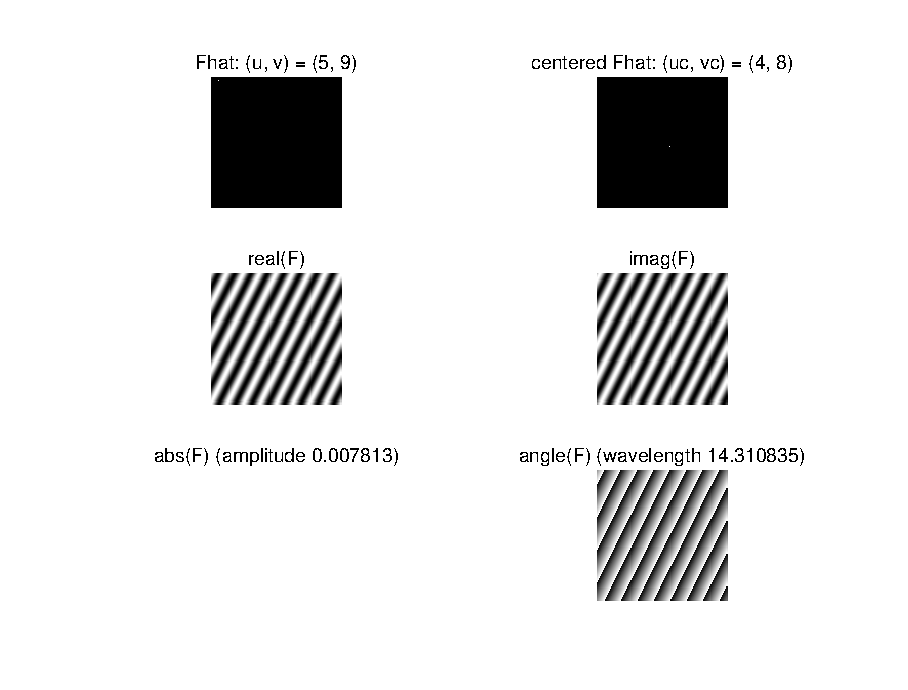
\includegraphics[width=0.9\columnwidth]{Q1_p_5_q_9.eps}
		\caption{$(p, q) = (5, 9)$.}
		\label{fig:Q1_p_5_q_9}
	\end{figure}
	\begin{figure}[!ht]
		\footnotesize
		\centering
		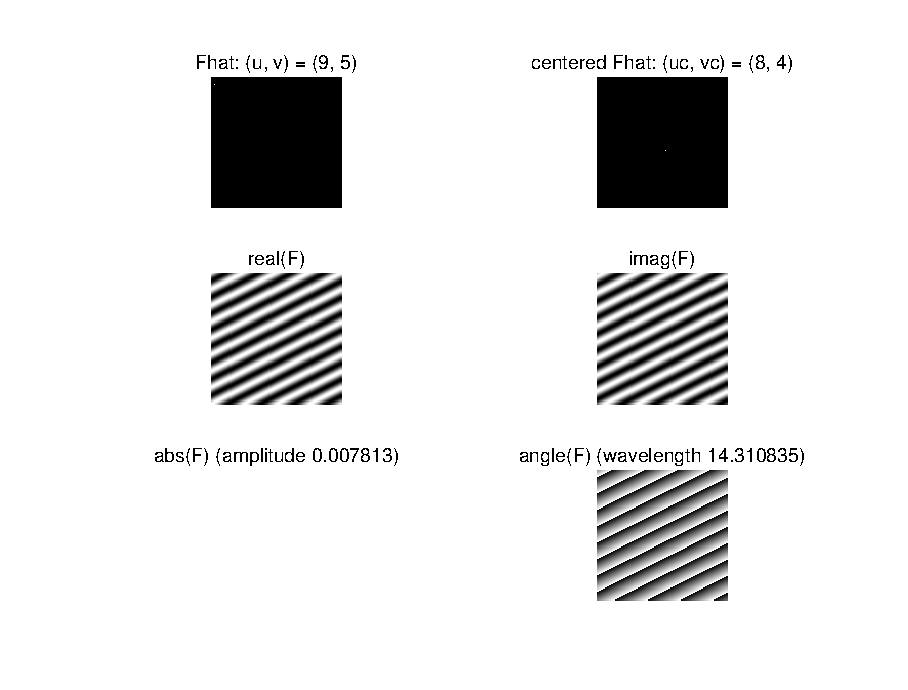
\includegraphics[width=0.9\columnwidth]{Q1_p_9_q_5.eps}
		\caption{$(p, q) = (9, 5)$.}
		\label{fig:Q1_p_9_q_5}
	\end{figure}
	\begin{figure}[!ht]
		\footnotesize
		\centering
		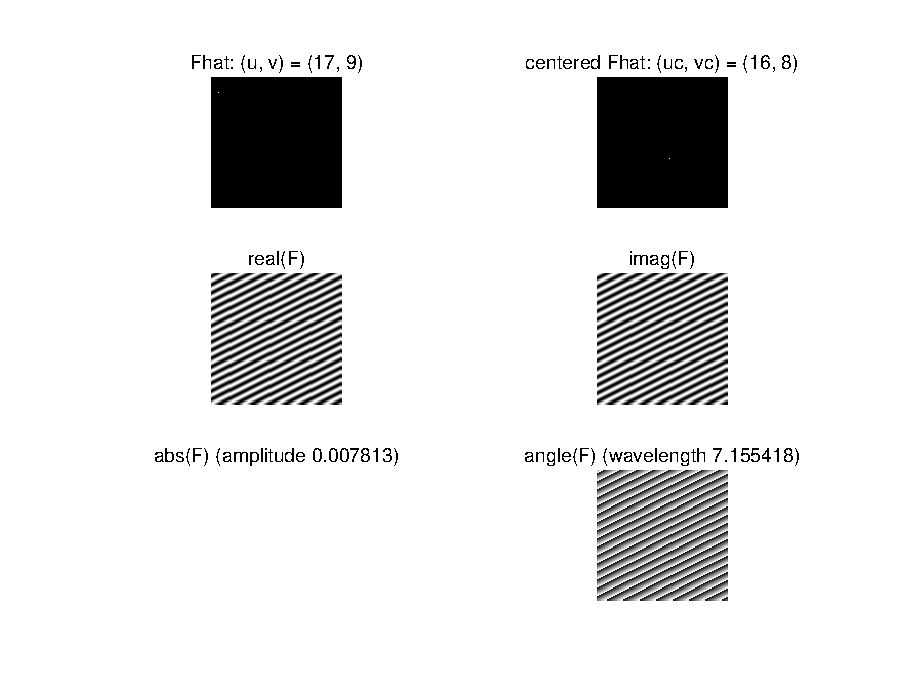
\includegraphics[width=0.9\columnwidth]{Q1_p_17_q_9.eps}
		\caption{$(p, q) = (17, 9)$.}
		\label{fig:Q1_p_17_q_9}
	\end{figure}
	\begin{figure}[!ht]
		\footnotesize
		\centering
		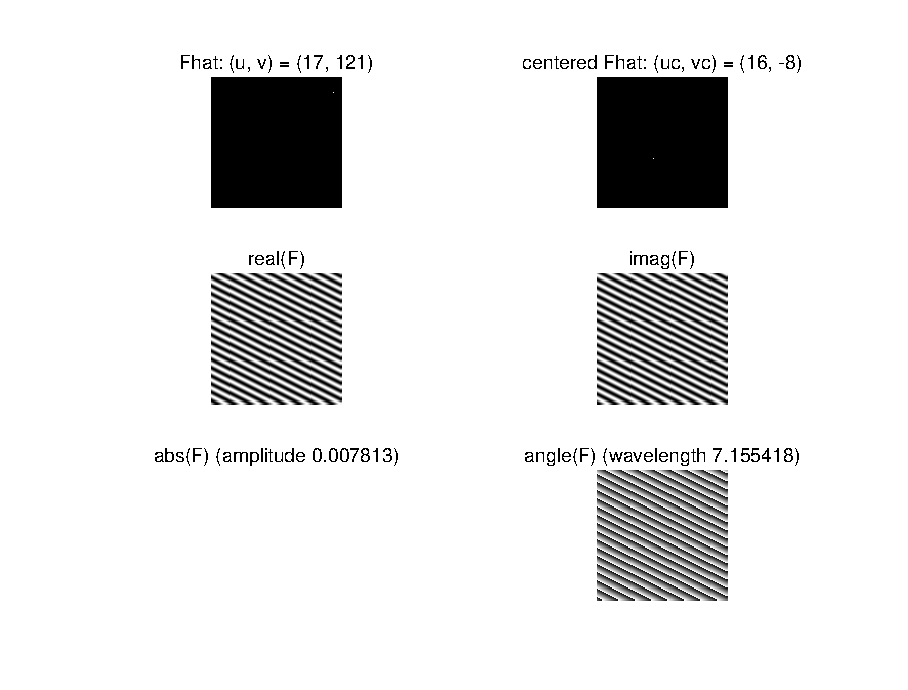
\includegraphics[width=0.9\columnwidth]{Q1_p_17_q_121.eps}
		\caption{$(p, q) = (17, 121)$.}
		\label{fig:Q1_p_17_q_121}
	\end{figure}
	\begin{figure}[!ht]
		\footnotesize
		\centering
		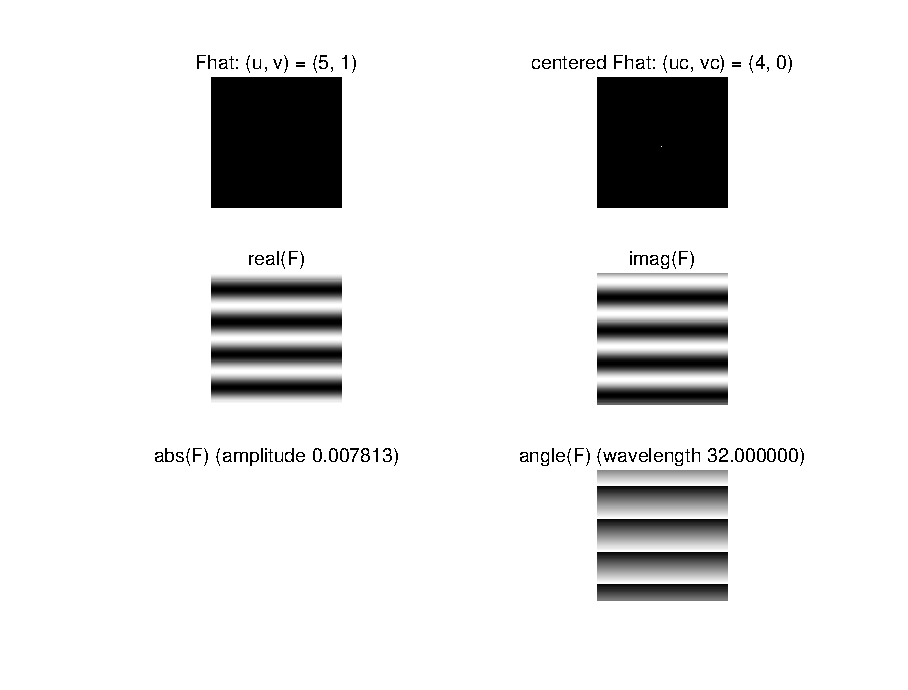
\includegraphics[width=0.9\columnwidth]{Q1_p_5_q_1.eps}
		\caption{$(p, q) = (5, 1)$.}
		\label{fig:Q1_p_5_q_1}
	\end{figure}
	\begin{figure}[!ht]
		\footnotesize
		\centering
		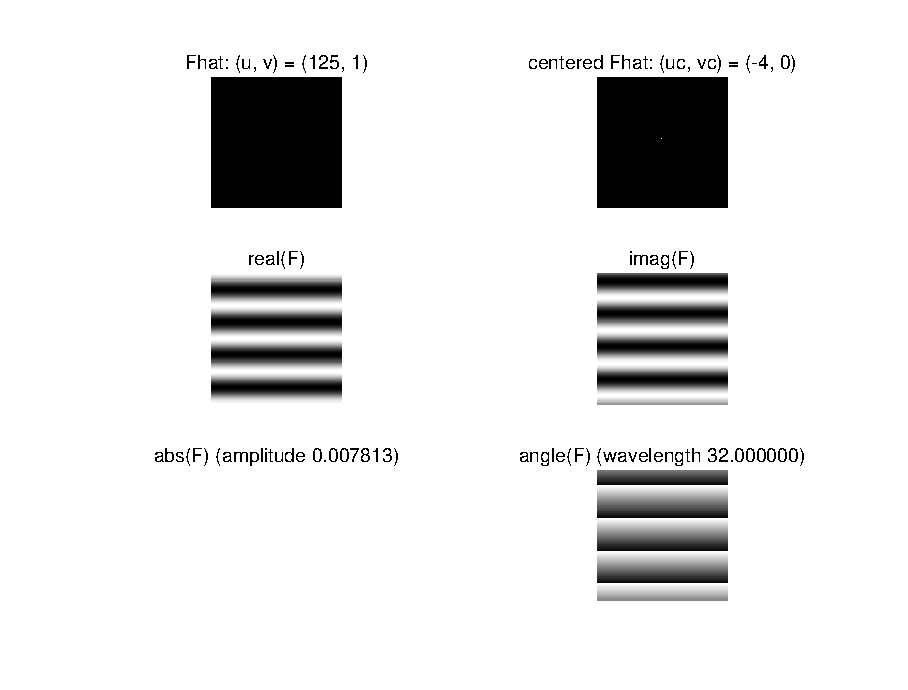
\includegraphics[width=0.9\columnwidth]{Q1_p_125_q_1.eps}
		\caption{$(p, q) = (125, 1)$.}
		\label{fig:Q1_p_125_q_1}
	\end{figure}

	\item \textbf{Question 2}: Explain how a position $(p,q)$ in the Fourier domain will be projected as a sine wave in the spatial domain. Illustrate with a MATLAB figure.
	\par The equation for the spatial domain is:
	\begin{align}
		f(x, y) &= \frac{1}{N}\sum_{x=0}^{N-1}\sum_{y=0}^{N-1}\delta(u-p, v-q) e^{\frac{2\pi i (xu + yv)}{N}} = \frac{1}{N}e^{\frac{2\pi i(px + qy)}{N}} \label{equ:spatial_domain}
	\end{align}
	\par The wavelength in $x$ direction and the wavelength in $y$ direction will determine the result of the sine wave in the spatial domain.

	\item \textbf{Question 3}: How large is the amplitude? Write down the expression derived from Equation (4) in these notes. Complement the code (variable \textbf{amplitude}) accordingly.
	\par As the spatial equation shown in Equation \ref{equ:spatial_domain}, the amplitude can be derived:
	\begin{align}
		\left|f(x, y)\right| &= \left|\frac{1}{N}e^{\frac{2\pi i(px + qy)}{N}}\right| = \frac{1}{N} \label{equ:amplitude}
	\end{align}

	\item \textbf{Question 4}: How does the direction and length of the sine wave depend on $p$ and $q$? Write down the explicit expression that can be found in the lecture notes. Complement the code (variable \textbf{wavelength}) accordingly.
	\par Base on the equation in the lecture slides:
	\begin{align}
		\lambda &= \frac{2\pi}{||\omega||} = \frac{2\pi}{\sqrt{\omega_{1}^{2}+\omega_{2}^{2}}} \\
		\omega &= \left[ \frac{2\pi u}{N} \frac{2\pi v}{N} \right]^{T} \label{equ:omega}
	\end{align}
	\par So the wavelength equation becomes:
	\begin{align}
		\lambda &= \frac{N}{\sqrt{p^{2}+q^{2}}} \label{equ:wavelength}
	\end{align}
	\par The direction could be obtained from the Equation \ref{equ:omega}, the angle will be \texttt{atan2($p, q$)} in MATLAB expression.

	\item \textbf{Question 5}: What happens when we pass the point in the center and either $p$ or $q$ exceeds half the image size? Explain and illustrate graphically with MATLAB!
	\par If either $p$ or $q$ exceeds half the image size which in this case is larger than 64, then the wavelength would be smaller than 2 according to Equation \ref{equ:wavelength}. When the period is 2, the spatial domain would be alternative black and white stripes of one-pixel-width. The corresponding maximum angular frequency is $\omega_{max} = \frac{2\pi}{2} = \pi$.
	\par When either $p$ or $q$ exceed $\frac{N}{2} = 64$, according to Equation \ref{equ:omega}, the angular frequency of $x$ or $y$ direction would exceed $\omega_{max}$, which means in such an quadratic image, the sinusoid wave could no longer be displayed. Figure \ref{fig:Q5_p_70_q_100} shows an example when $(p, q) = (70, 100)$.
	\begin{figure}[!ht]
		\footnotesize
		\centering
		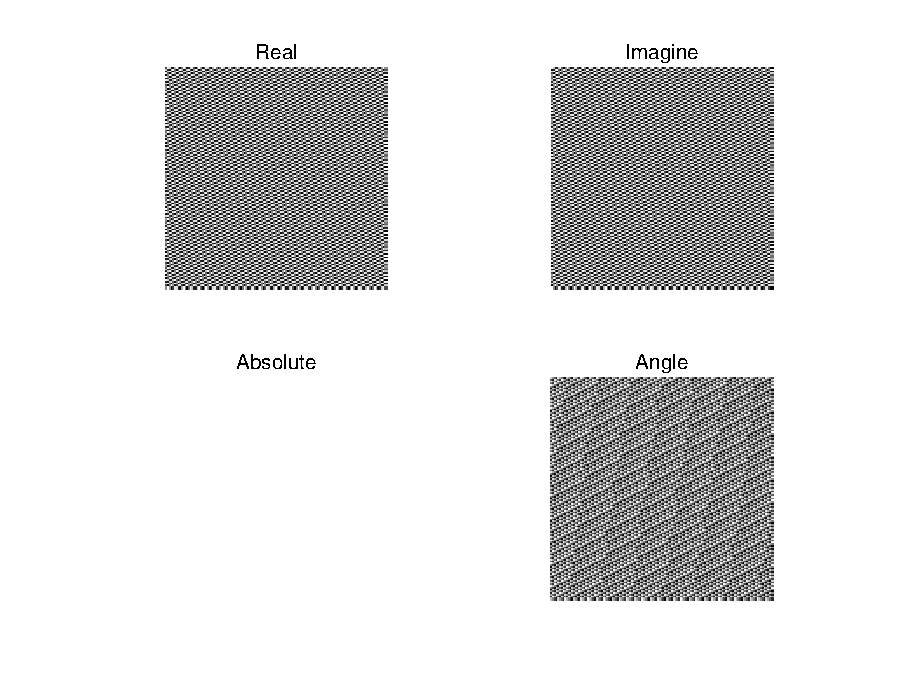
\includegraphics[width=0.8\columnwidth]{Q5_p_70_q_100.eps}
		\caption{$(p, q) = (70, 100)$.}
		\label{fig:Q5_p_70_q_100}
	\end{figure}

	\item \textbf{Question 6}: What is the purpose of the instructions following the question \texttt{What is done by these instructions?} in the code?
	\par The purpose of the code following after \texttt{What is done by these instructions?} is to shift the Fourier function so that the angular frequency in $x$ and $y$ direction could be inside $\left[-\pi, \pi\right]$, which can be also implemented by MATLAB function \texttt{fftshift}. Also, this part of code make the origin point move from $(1, 1)$ to $(0, 0)$.
\end{itemize}

\subsection*{1.4 Linearity}
\par The origin figure of F, G, and H are shown in Figure \ref{fig:F}, \ref{fig:G}, and \ref{fig:H} accordingly. Their Fourier transform and other operations are shown in Figure \ref{fig:spactrum}, \ref{fig:shiftedSpactrum}, and \ref{fig:shiftedSpactrumNoLog}.
\begin{figure}[!ht]
	\footnotesize
	\centering 
	\begin{subfigure}[t]{.32\linewidth} % .32 for three polts .49 for two plots
	
\includegraphics[width=\columnwidth]{Linearity_F.eps}
	\caption{Image F}
	\label{fig:F}
	\end{subfigure}
	\begin{subfigure}[t]{.32\linewidth} % .32 for three polts
	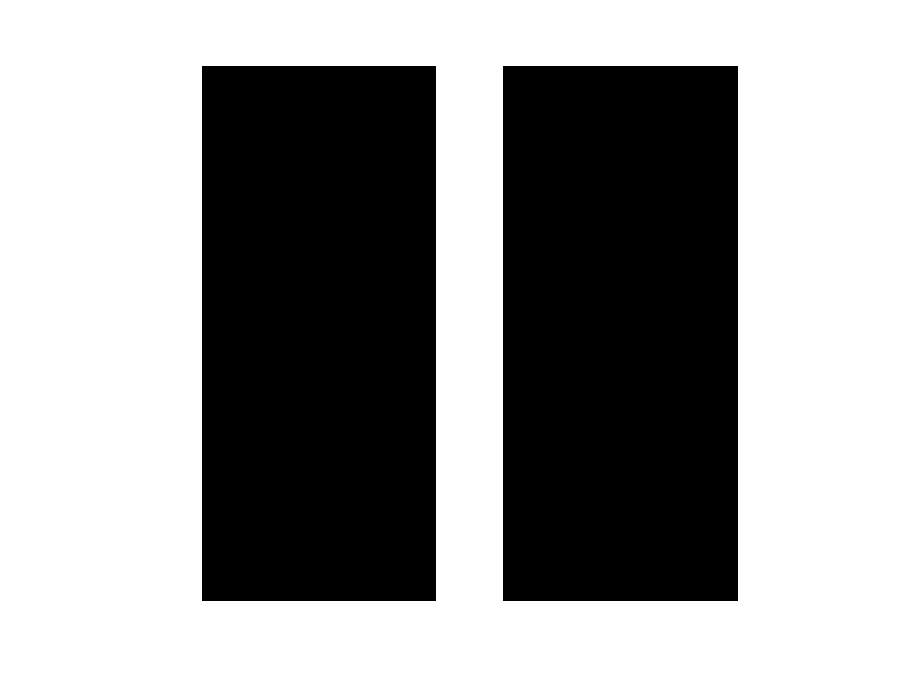
\includegraphics[width=\columnwidth]{Linearity_G.eps}
	\caption{Image G = F'}
	\label{fig:G}
	\end{subfigure}
	\begin{subfigure}[t]{.32\linewidth} % .32 for three polts
	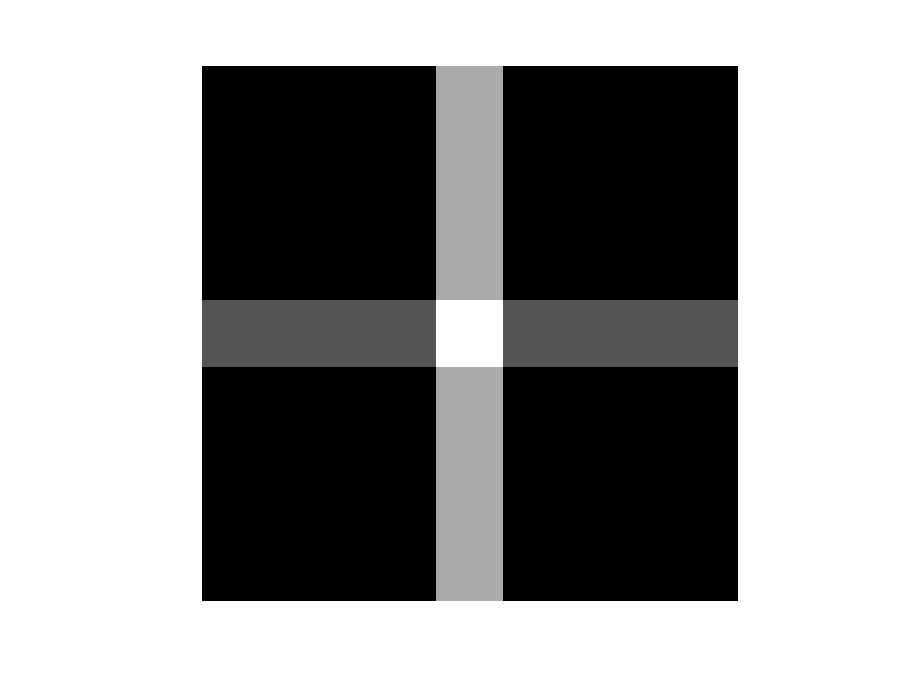
\includegraphics[width=\columnwidth]{Linearity_H.eps}
	\caption{Image H = F + 2 * G}
	\label{fig:H}
	\end{subfigure}
	\caption{Origin images.}
	\label{fig:origin}
\end{figure}

\begin{figure}[!ht]
	\footnotesize
	\centering 
	\begin{subfigure}[t]{.32\linewidth} % .32 for three polts .49 for two plots
	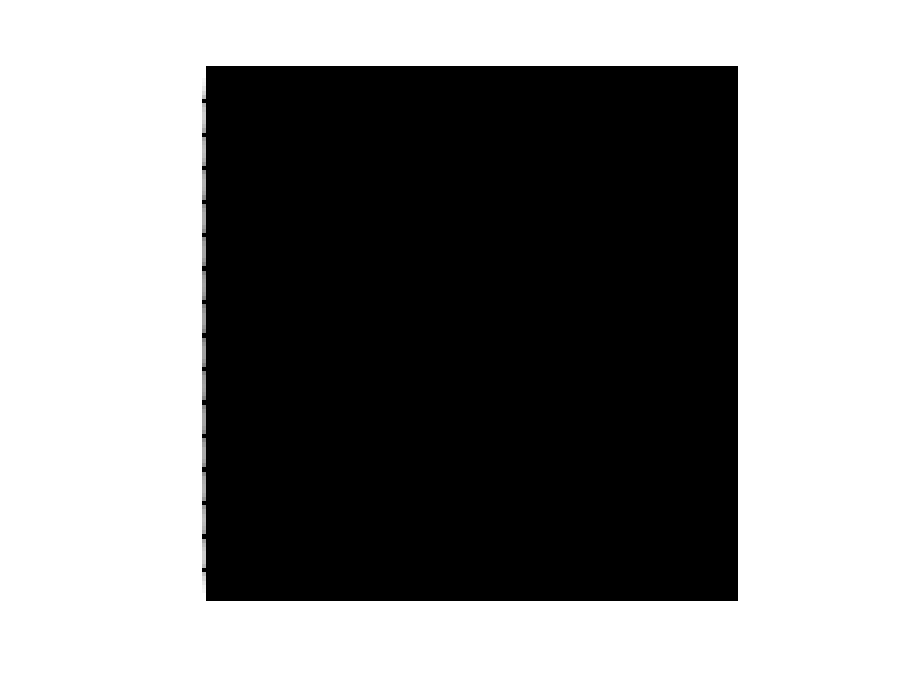
\includegraphics[width=\columnwidth]{Linearity_Fhat_Abs_Log.eps}
	\caption{Fourier spectra of F.}
	\label{fig:Fhat_Abs_Log}
	\end{subfigure}
	\begin{subfigure}[t]{.32\linewidth} % .32 for three polts .49 for two plots
	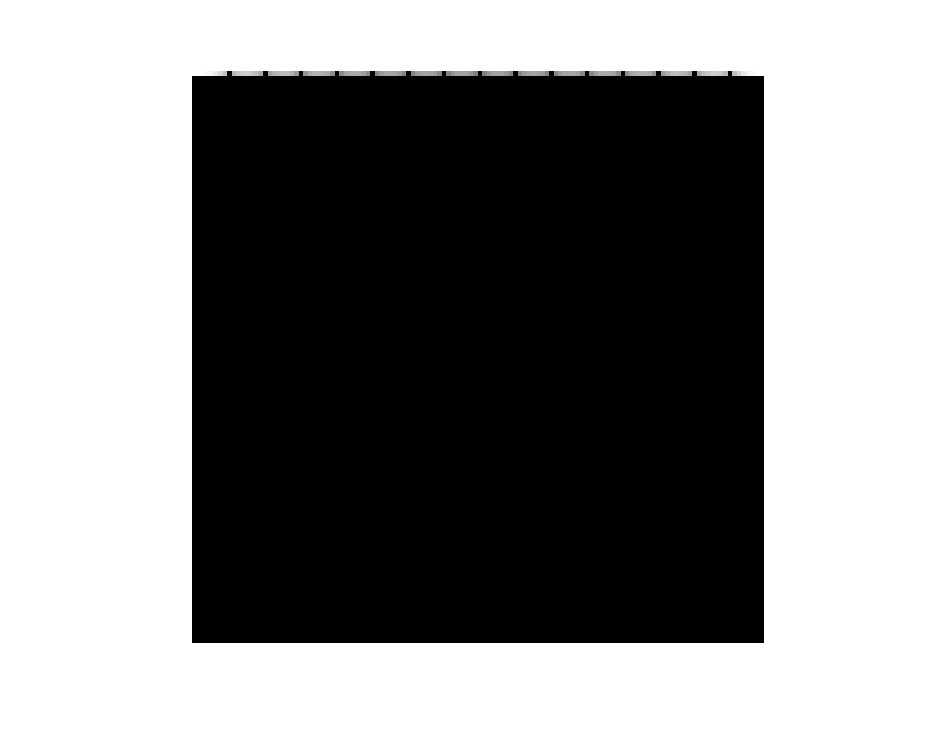
\includegraphics[width=.95\columnwidth]{Linearity_Ghat_Abs_Log.eps}
	\caption{Fourier spectra of G.}
	\label{fig:Ghat_Abs_Log}
	\end{subfigure}
	\begin{subfigure}[t]{.32\linewidth} % .32 for three polts .49 for two plots
	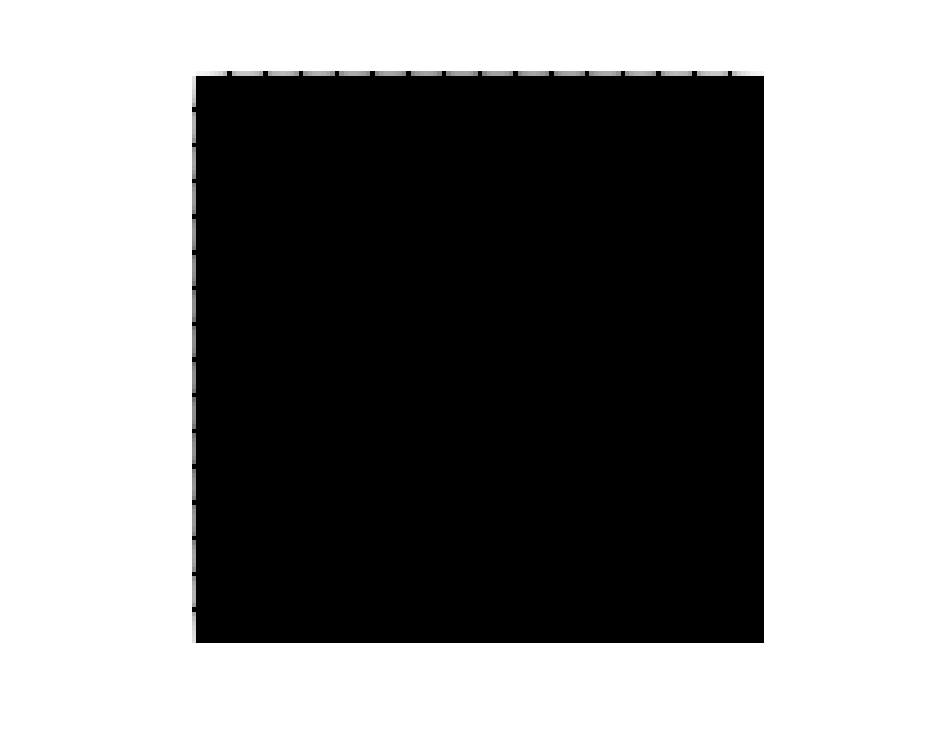
\includegraphics[width=.95\columnwidth]{Linearity_Hhat_Abs_Log.eps}
	\caption{Fourier spectra of H.}
	\label{fig:Hhat_Abs_Log}
	\end{subfigure}
	\caption{Fourier spectra originated at upper left corner.}
	\label{fig:spactrum}
\end{figure}

\begin{figure}[!ht]
	\footnotesize
	\centering 
	\begin{subfigure}[t]{.32\linewidth} % .32 for three polts .49 for two plots
		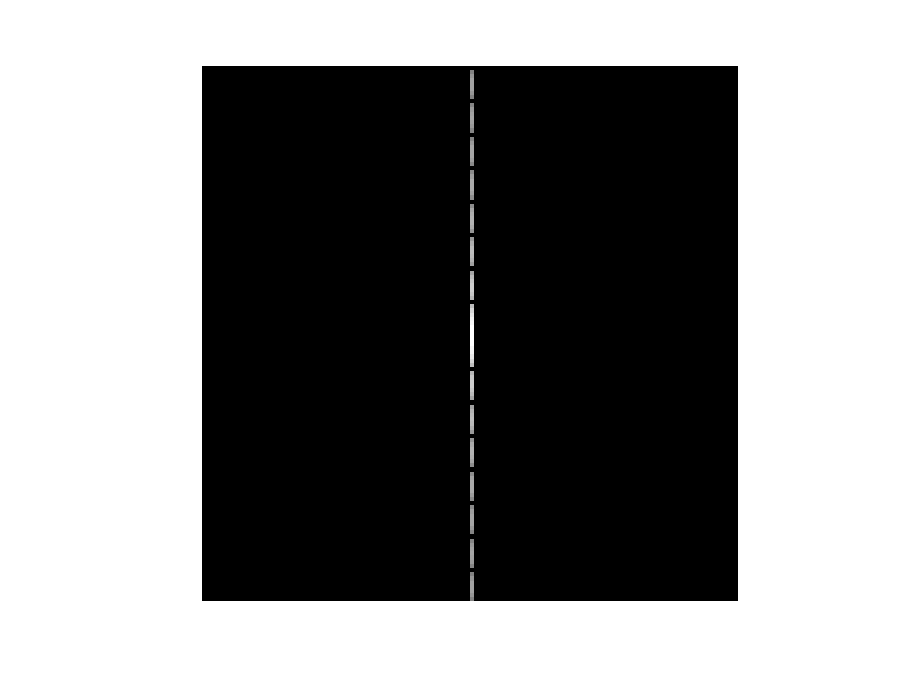
\includegraphics[width=\columnwidth]{Linearity_Fhat_Shift_Abs_Log.eps}
		\caption{Shifted Fourier spectra of F.}
		\label{fig:Fhat_Shift_Abs_Log}
	\end{subfigure}
	\begin{subfigure}[t]{.32\linewidth} % .32 for three polts .49 for two plots
		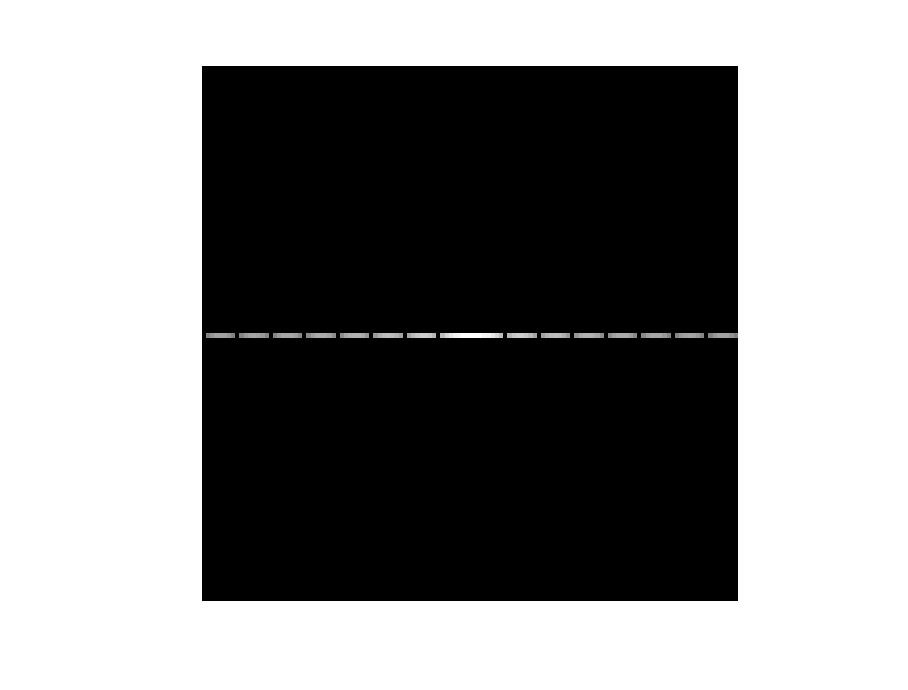
\includegraphics[width=\columnwidth]{Linearity_Ghat_Shift_Abs_Log.eps}
		\caption{Shifted Fourier spectra of G.}
		\label{fig:Ghat_Shift_Abs_Log}
	\end{subfigure}
	\begin{subfigure}[t]{.32\linewidth} % .32 for three polts .49 for two plots
		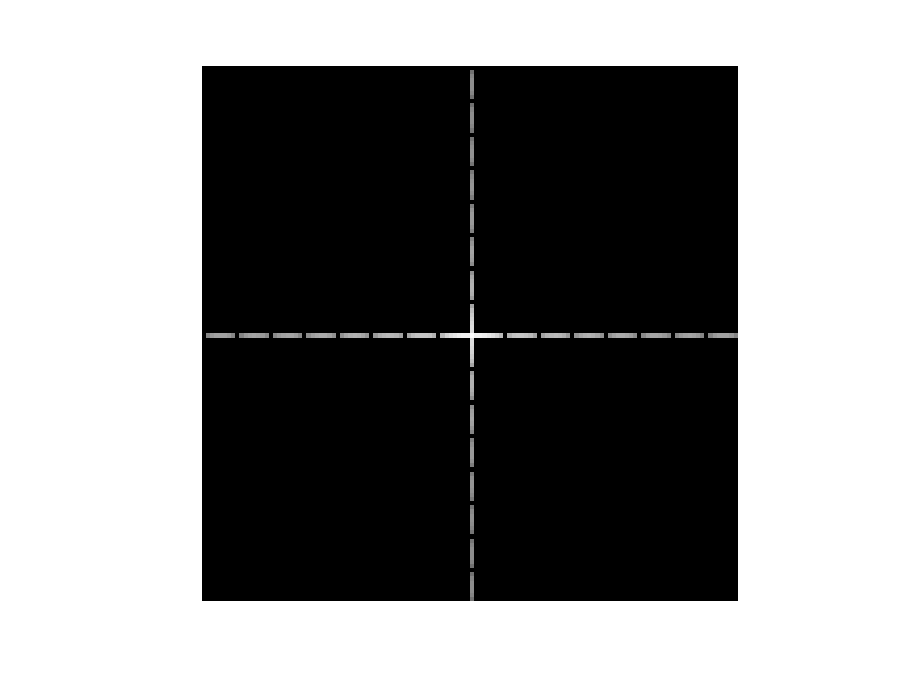
\includegraphics[width=\columnwidth]{Linearity_Hhat_Shift_Abs_Log.eps}
		\caption{Shifted Fourier spectra of H.}
		\label{fig:Hhat_Shift_Abs_Log}
	\end{subfigure}
	\caption{Fourier spectra originated at middle.}
	\label{fig:shiftedSpactrum}
\end{figure}

\begin{figure}[!ht]
	\footnotesize
	\centering 
	\begin{subfigure}[t]{.32\linewidth} % .32 for three polts .49 for two plots
	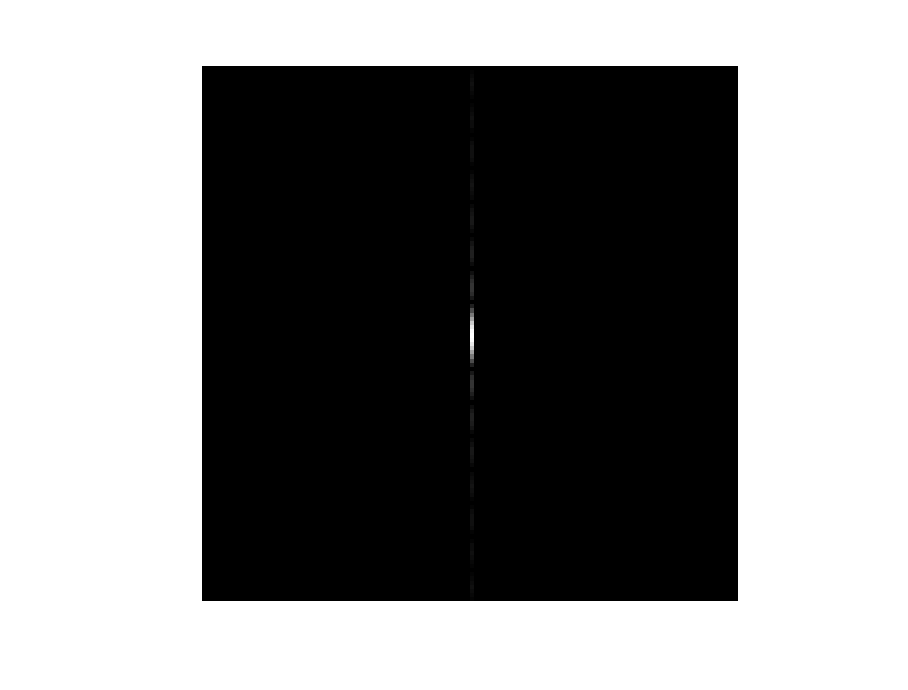
\includegraphics[width=\columnwidth]{Linearity_Fhat_Shift_Abs.eps}
	\caption{Shifted Fourier spectra of F without \texttt{Log}.}
	\label{fig:Fhat_Shift_Abs}
	\end{subfigure}
	\begin{subfigure}[t]{.32\linewidth} % .32 for three polts .49 for two plots
	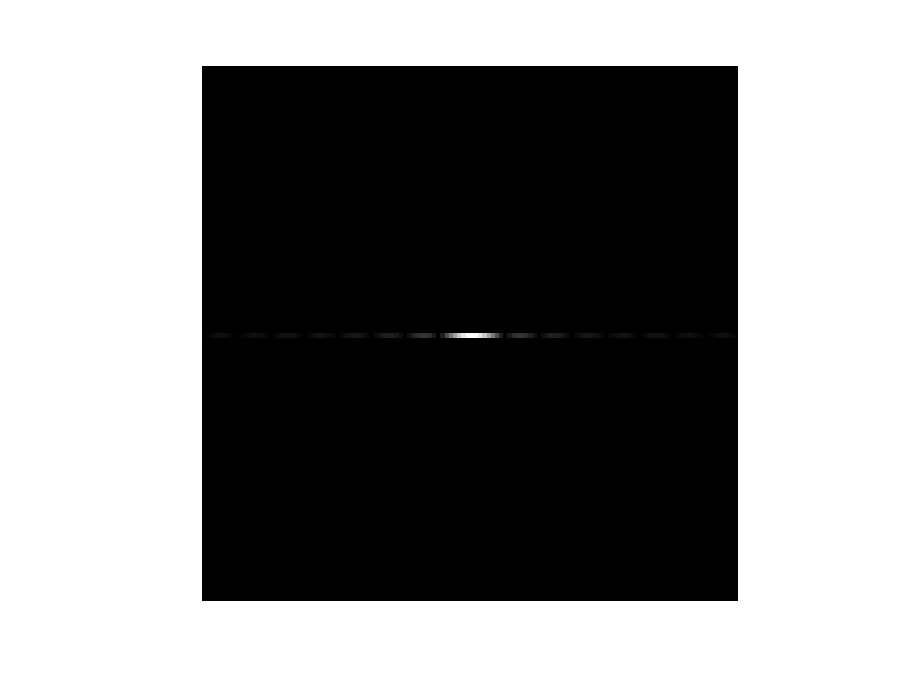
\includegraphics[width=\columnwidth]{Linearity_Ghat_Shift_Abs.eps}
	\caption{Shifted Fourier spectra of G without \texttt{Log}.}
	\label{fig:Ghat_Shift_Abs}
	\end{subfigure}
	\begin{subfigure}[t]{.32\linewidth} % .32 for three polts .49 for two plots
	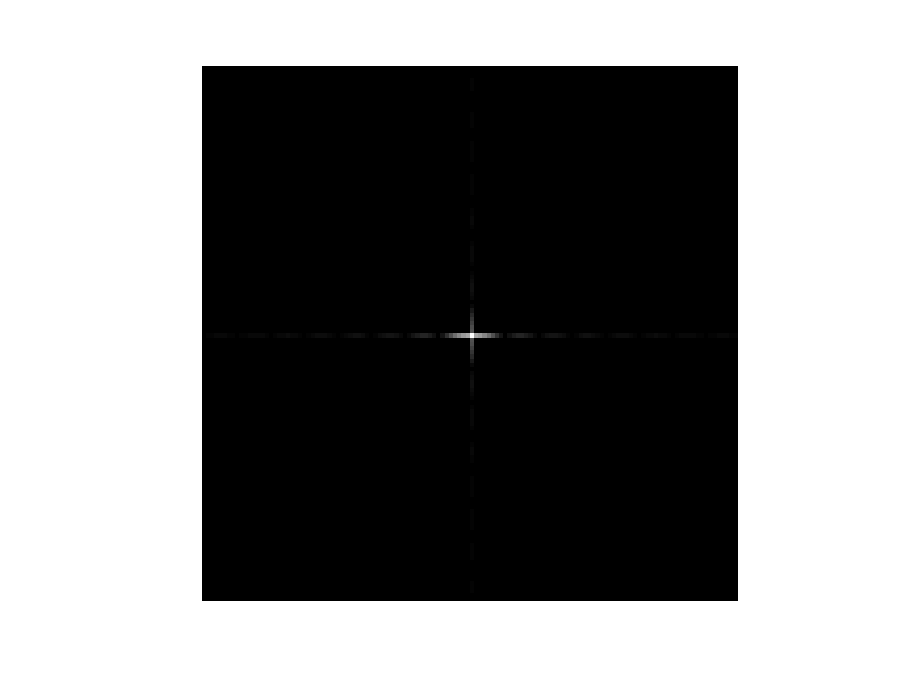
\includegraphics[width=\columnwidth]{Linearity_Hhat_Shift_Abs.eps}
	\caption{Shifted Fourier spectra of H without \texttt{Log}.}
	\label{fig:Hhat_Shift_Abs}
	\end{subfigure}
	\caption{Fourier spectra originated at middle without \texttt{Log}.}
	\label{fig:shiftedSpactrumNoLog}
\end{figure}

\begin{itemize}
	\item \textbf{Question 7} Why are these Fourier spectra concentrated to the borders of the images? Can you give a mathematical interpretation? Hint: think of the frequencies in the source image and consider the resulting image as a Fourier transform applied to a 2D function. It might be easier to analyze each dimension separately!
	\par The function of F in this case could be written as $F(x, y) = 1$ for all $y \in \left[y_{1}, y_{2}\right]$ and equals to $0$ otherwise. Then we will have:
	\begin{align}
		\mathcal{F}(u, v) &= \frac{1}{N}\sum_{x=0}^{N-1}\sum_{y=0}^{N-1}F(x,y)e^{-\frac{2\pi i(xu+yv)}{N}} \\
		&= \frac{1}{N}\sum_{x=0}^{N-1}\sum_{y=y_{1}}^{y_{2}}e^{-\frac{2\pi i(xu+yv)}{N}} \\
		&= \frac{1}{N}\sum_{y=y_{1}}^{y_{2}}e^{-\frac{2\pi iyv}{N}}\sum_{x=0}^{N-1}e^{-\frac{2\pi ixu}{N}} \\
		&= \frac{\delta(u)}{N}\sum_{y=y_{1}}^{y_{2}}e^{-\frac{2\pi iyv}{N}} \label{equ:Q_7_F}
	\end{align}
	\par Based on Equation \ref{equ:Q_7_F}, we can see that only when $u=0$ that the Fourier spectra of image F would not be zero, which means the Fourier spectra of F would be concentrated to the left border. Sample reason could be applied to G to explain why the Fourier spectra is concentrated to the up border of the image. As for H, since H is a linear combination of F and G, the Fourier spectra of H would also be a linear combination of the Fourier spectrum of F and G, which gives Figure \ref{fig:Hhat_Abs_Log}.
	
	\item \textbf{Question 8} Why is the logarithm function applied?
	\par The logarithm function is applied to making the difference between each pixels smaller, so that enhance the dark parts in Figure \ref{fig:shiftedSpactrumNoLog}, and making them being seen clearly as shown in Figure \ref{fig:shiftedSpactrum}.
	
	\item \textbf{Question 9} What conclusions can be drawn regarding linearity? From your observations can you derive a mathematical expression in the general case?
	\par Comparing Figure \ref{fig:Hhat_Shift_Abs_Log} with Figure \ref{fig:Fhat_Shift_Abs_Log} and \ref{fig:Ghat_Shift_Abs_Log}, we can find that shifted Fourier spectra of H is a linear combination of the one of F and G. In general, the expression of this property could be written as:
	\begin{align}
		\mathcal{F}[\alpha g(x, y) + \beta h(x, y)] = \alpha \mathcal{G}(u, v) + \beta \mathcal{H}(u, v) \label{equ:linearity}
	\end{align}
\end{itemize}

\subsection*{1.5 Multiplication}
\par In this section, image F is Figure \ref{fig:F} and image G is Figure \ref{fig:G}.
\begin{itemize}
	\item \textbf{Question 10} Are there any other ways to compute the last image? \textbf{Remember what multiplication in Fourier domain equals to in the spatial domain!} Perform these alternative computations in practice.
	\par Based on the convolution theory of Fourier transform, we have such equation:
	\begin{align}
		\mathcal{F}[H(x,y) \times G(x,y)] = \mathcal{H}(u,v) * \mathcal{G}(u,v) \label{equ:convolutionTheory}
	\end{align}
	\begin{figure}[!ht]
		\centering 
		\begin{subfigure}[t]{.32\linewidth} % .32 for three polts .49 for two plots
		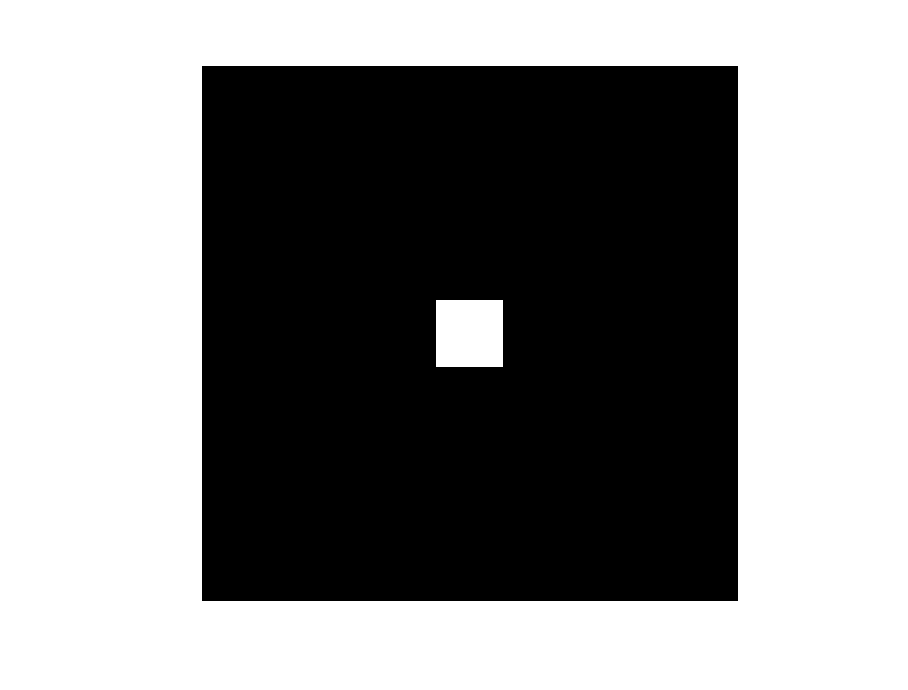
\includegraphics[width=\columnwidth]{Multiplication_F_G.eps}
		\caption{\scriptsize Multiplication of F and G.}
		\label{fig:F*G}
		\end{subfigure}
		\begin{subfigure}[t]{.32\linewidth} % .32 for three polts .49 for two plots
		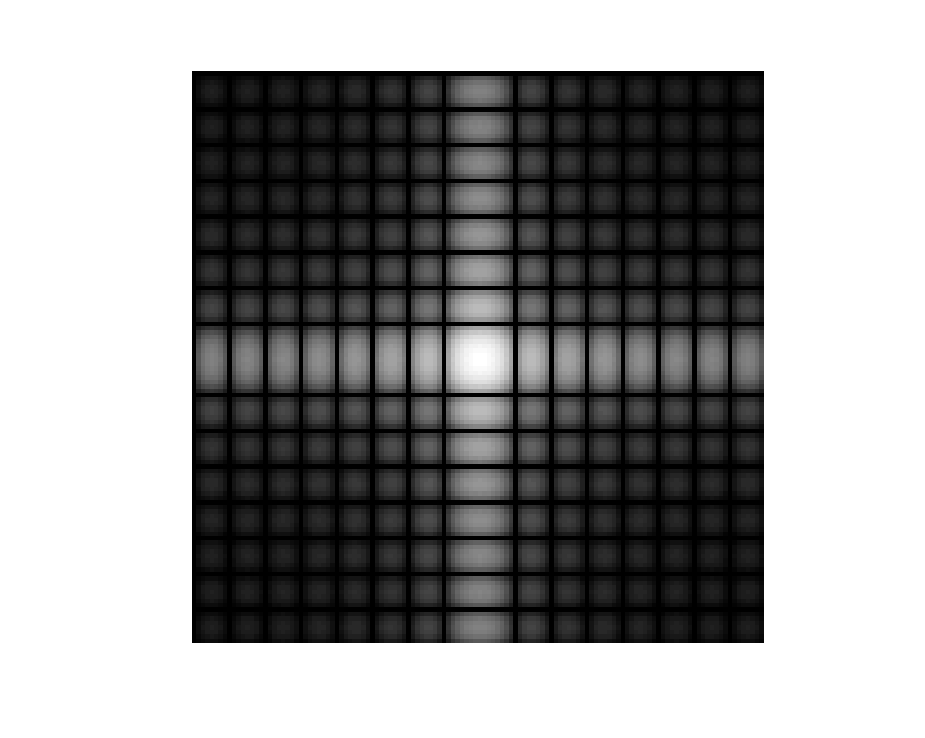
\includegraphics[width=0.95\columnwidth]{Multiplication_Shifted_Fourier_F_G.eps}
		\caption{\scriptsize Shifted Fourier spectra of multiplication of F and G.}
		\label{fig:shiftedFourierF*G}
		\end{subfigure}
		\begin{subfigure}[t]{.32\linewidth} % .32 for three polts .49 for two plots
		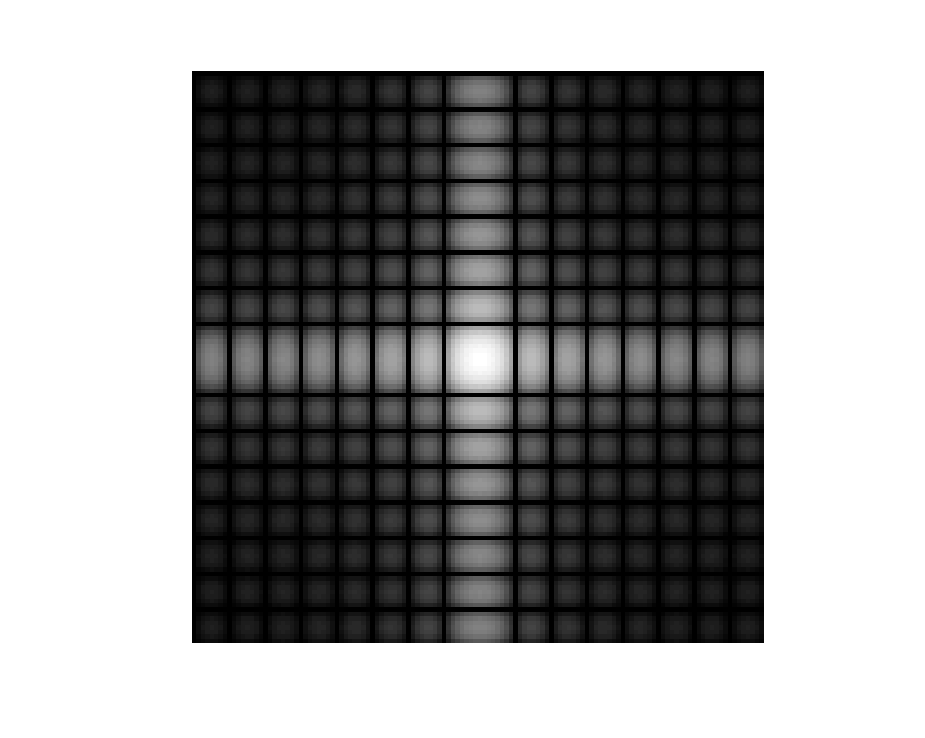
\includegraphics[width=0.95\columnwidth]{Multiplication_Shifted_Fourier_Convolution_F_G.eps}
		\caption{\scriptsize Shifted Fourier spectra of convolution of $\mathcal{F}$ and $\mathcal{G}$.}
		\label{fig:shiftedConvolutionF*G}
		\end{subfigure}
		\caption{Convolution.}
	\end{figure}
	\par So, we can convolute $\mathcal{F}$ and $\mathcal{H}$ in the Fourier domain. Since \texttt{fft2} in MATLAB uses 1 as factor in the FFT-routine, we divide the convolution result by $N^{2}$. Also, the convolution would give a $255\times 255$ matrix for the result, so we would only use the $128\times 128$ matrix at the left upper corner. And finally we could get the shifted Fourier spectra as Figure \ref{fig:shiftedConvolutionF*G} which is same to Figure \ref{fig:shiftedFourierF*G}, the result given by multiplication and then Fourier transformation.
\end{itemize}

\subsection*{1.6 Scaling}
\begin{itemize}
	\item \textbf{Question 11} What conclusions can be drawn from comparing the results with those in the previous exercise? See how the source images have changed and analyze the effects of scaling.
	\par Image F and its Fourier transform are illustrated in Figure \ref{fig:scaledF} and \ref{fig:shiftedFourierScaledF} respectively.
	\begin{figure}[!ht]
		\scriptsize
		\centering 
		\begin{subfigure}[t]{.49\linewidth} % .32 for three polts .49 for two plots
		
\includegraphics[width=\columnwidth]{Scaling_F.eps}
		\caption{\scriptsize Scaled F.}
		\label{fig:scaledF}
		\end{subfigure}
		\begin{subfigure}[t]{.49\linewidth} % .32 for three polts .49 for two plots
		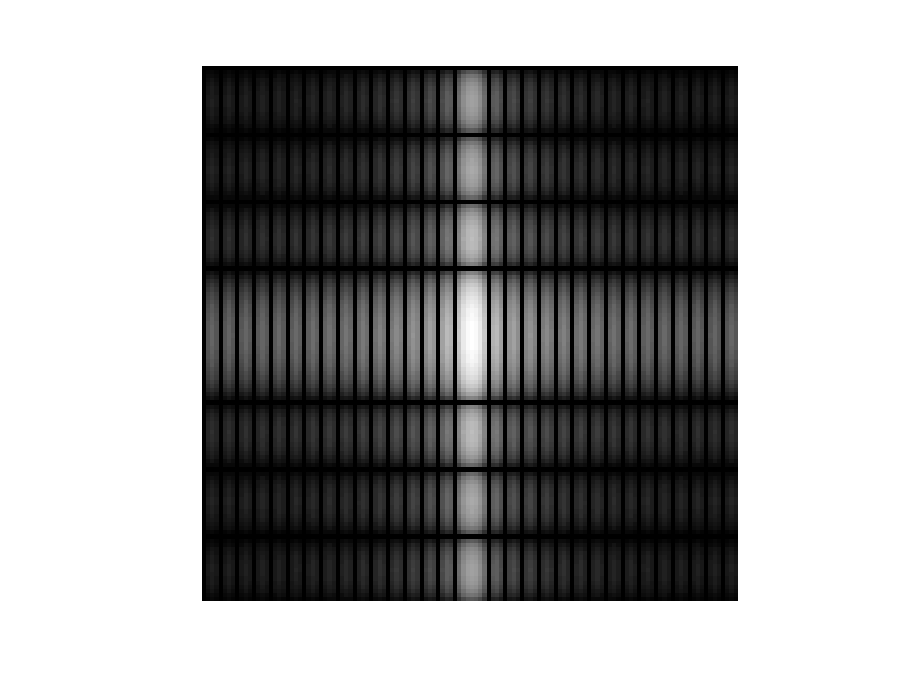
\includegraphics[width=0.95\columnwidth]{Scaling_F_Shifted_Log_Fourier.eps}
		\caption{\scriptsize Shifted Fourier spectra of scaled F.}
		\label{fig:shiftedFourierScaledF}
		\end{subfigure}
		\caption{Scaling.}
	\end{figure}
	\par Comparing to Figure \ref{fig:F*G} and \ref{fig:shiftedFourierF*G}, we can see that F in Figure \ref{fig:scaledF} is a scaled version of Figure \ref{fig:F*G} which is half of its height and double of this width. While Figure \ref{fig:shiftedFourierScaledF} is stretched in height and compressed in width when comparing to Figure \ref{fig:shiftedFourierF*G}. The scaling property of discrete Fourier transform can be derived as Equation \ref{equ:scalingProperty}.
	\begin{align}
		\mathcal{F}[G(\alpha x, \beta y)] = \frac{1}{|\alpha\beta|}\mathcal{G}(\frac{u}{\alpha}, \frac{v}{\beta}) \label{equ:scalingProperty}
	\end{align}
	\par Since $F_{2}(x, y) = F_{1}(\frac{x}{2}, 2y)$, $\mathcal{F}_{2}(u, v) = \mathcal{F}_{1}(2u, \frac{v}{2})$.
\end{itemize}

\subsection*{1.7 Rotation}
\begin{itemize}
	\item \textbf{Question 12} What can be said about possible similarities and differences? Hint: think of the frequencies and how they are affected by the rotation.
	\par The original image of F and its shifted Fourier with logarithm function are illustrated in Figure \ref{fig:scaledF} and \ref{fig:shiftedFourierScaledF}. The rotated image of F, their Fourier spectrum, and their rotated back Fourier spectrum with rotation angle varies from $30^{\circ}$, $60^{\circ}$, and $90^{\circ}$ are illustrated in Figure \ref{fig:rotation}.
	\begin{figure}[!ht]
		\footnotesize
		\centering 
		\begin{subfigure}[t]{.32\linewidth} % .32 for three polts .49 for two plots
		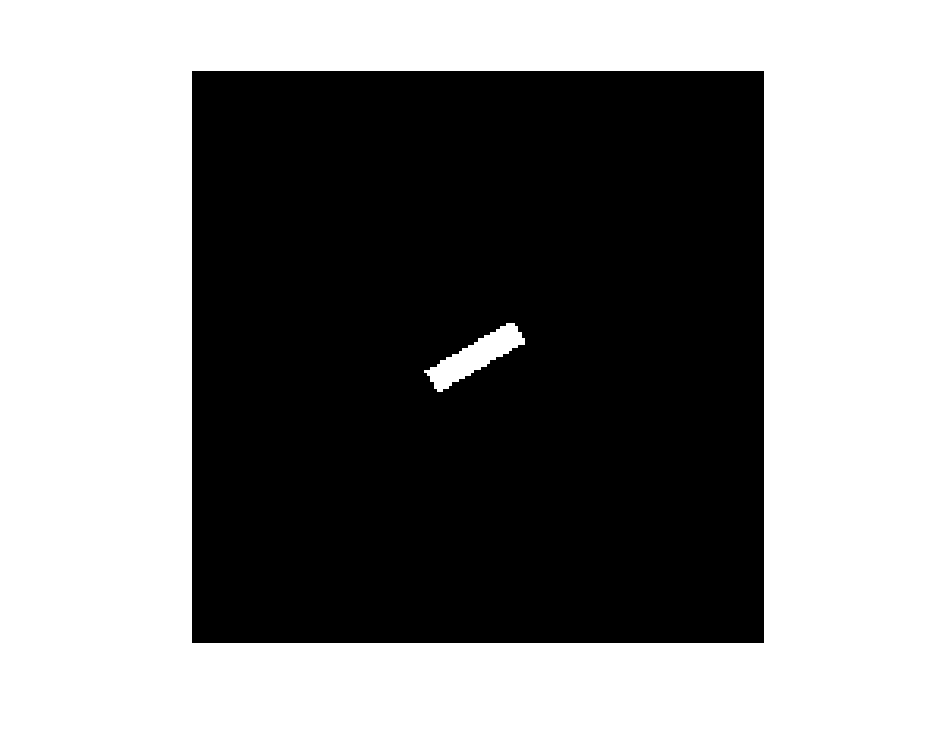
\includegraphics[width=\columnwidth]{Rotation_G_30.eps}
		\caption{\scriptsize Rotated by $30^{\circ}$.}
		\label{fig:rotated30}
		\end{subfigure}
		\begin{subfigure}[t]{.32\linewidth} % .32 for three polts .49 for two plots
		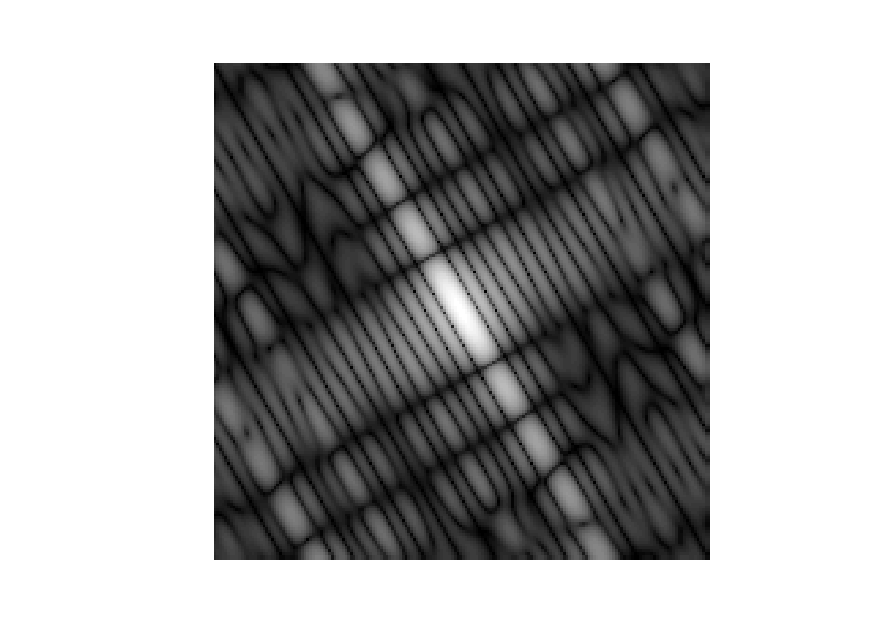
\includegraphics[width=\columnwidth]{Rotation_G_30_Shifted_Fourier.eps}
		\caption{\scriptsize Fourier transform with $30^{\circ}$ rotation.}
		\label{fig:rotated30Fourier}
		\end{subfigure}
		\begin{subfigure}[t]{.32\linewidth} % .32 for three polts .49 for two plots
		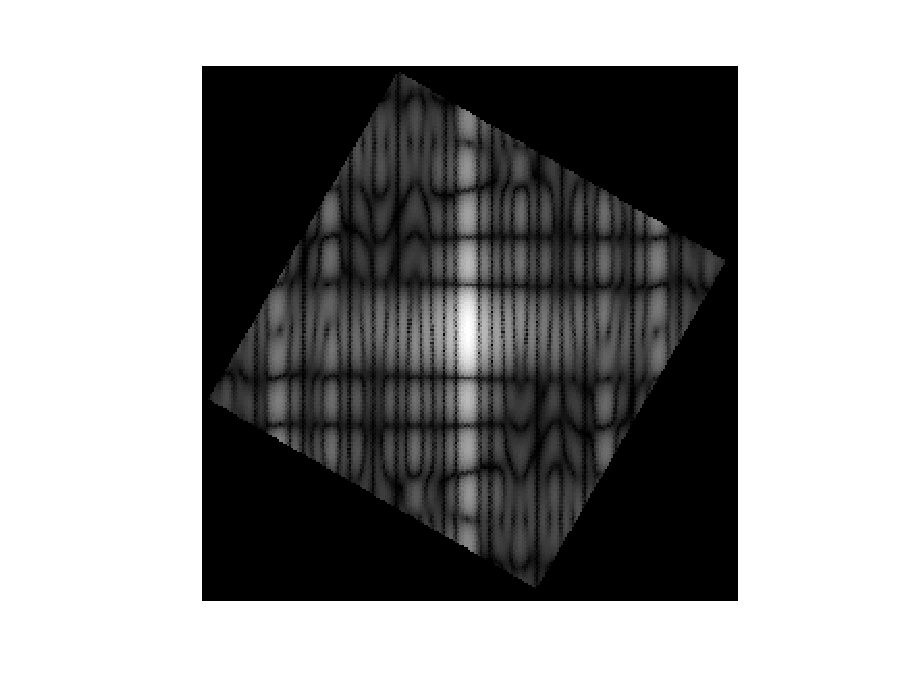
\includegraphics[width=\columnwidth]{Rotation_G_30_Fourier_Back.eps}
		\caption{\scriptsize Image rotated back by $30^{\circ}$.}
		\label{fig:rotated30Back}
		\end{subfigure}
		
		\begin{subfigure}[t]{.32\linewidth} % .32 for three polts .49 for two plots
		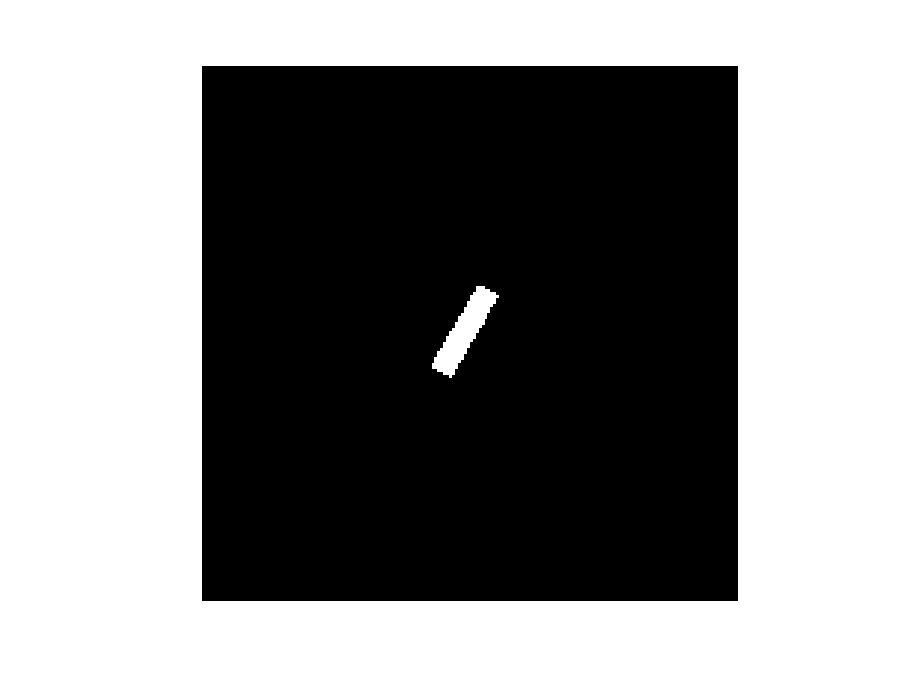
\includegraphics[width=\columnwidth]{Rotation_G_60.eps}
		\caption{\scriptsize Rotated by $60^{\circ}$.}
		\label{fig:rotated60}
		\end{subfigure}
		\begin{subfigure}[t]{.32\linewidth} % .32 for three polts .49 for two plots
		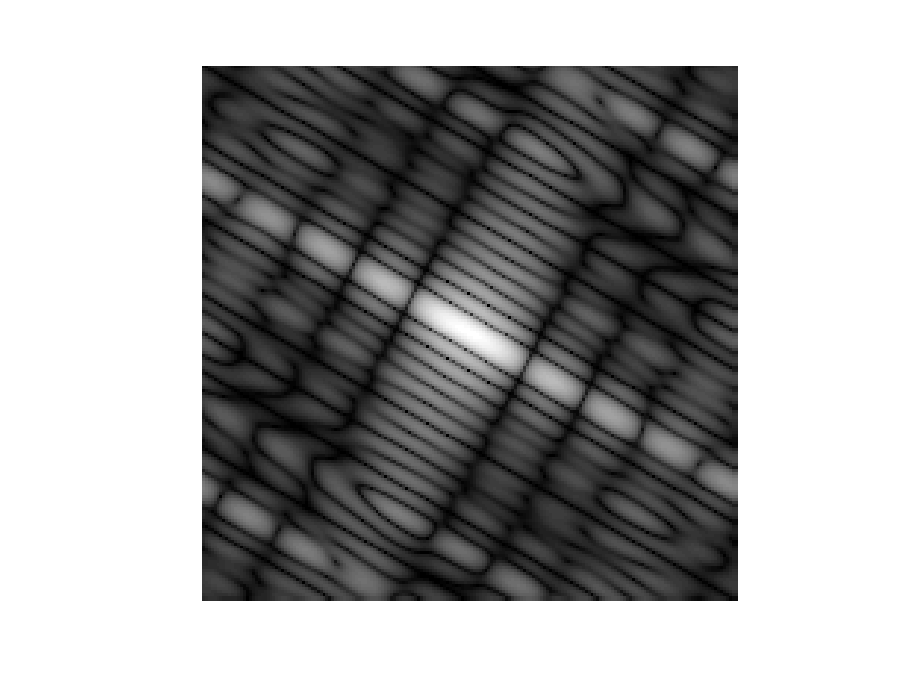
\includegraphics[width=\columnwidth]{Rotation_G_60_Shifted_Fourier.eps}
		\caption{\scriptsize Fourier transform with $60^{\circ}$ rotation.}
		\label{fig:rotated60Fourier}
		\end{subfigure}
		\begin{subfigure}[t]{.32\linewidth} % .32 for three polts .49 for two plots
		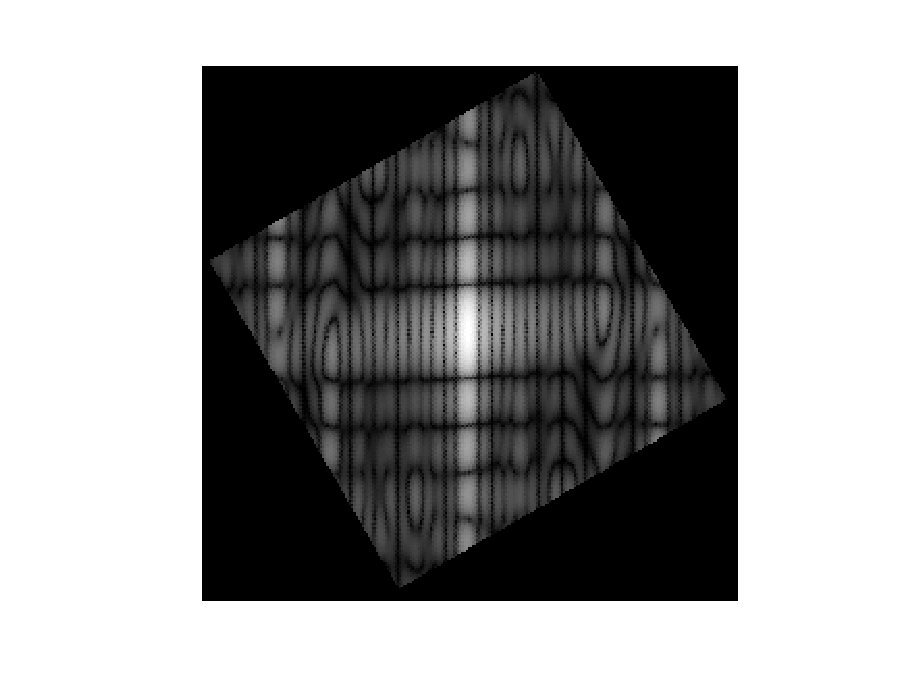
\includegraphics[width=\columnwidth]{Rotation_G_60_Fourier_Back.eps}
		\caption{\scriptsize Image rotated back by $60^{\circ}$.}
		\label{fig:rotated60Back}
		\end{subfigure}
		
		\begin{subfigure}[t]{.32\linewidth} % .32 for three polts .49 for two plots
		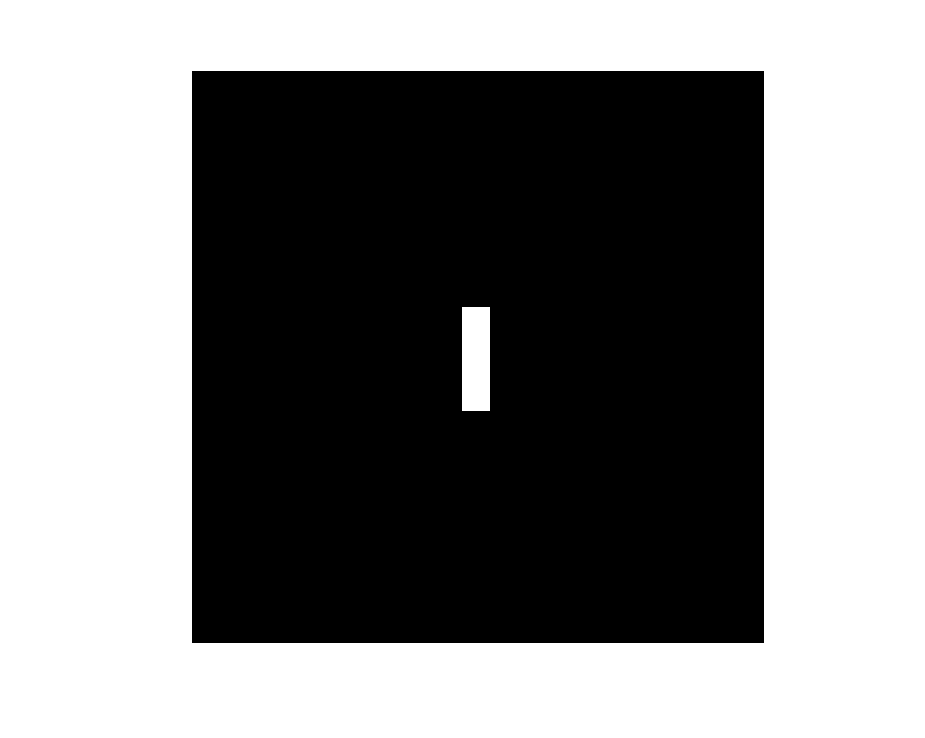
\includegraphics[width=\columnwidth]{Rotation_G_90.eps}
		\caption{\scriptsize Rotated by $90^{\circ}$.}
		\label{fig:rotated90}
		\end{subfigure}
		\begin{subfigure}[t]{.32\linewidth} % .32 for three polts .49 for two plots
		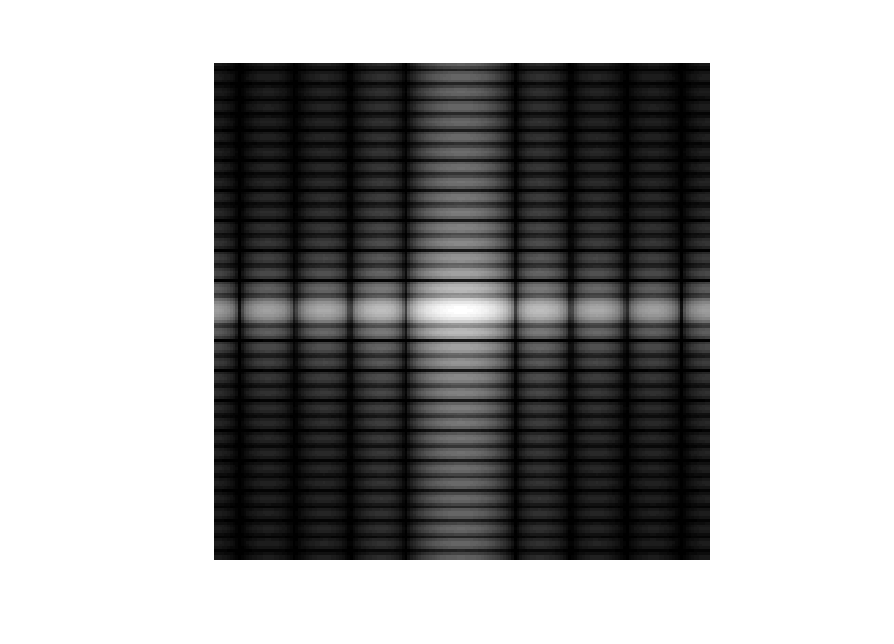
\includegraphics[width=\columnwidth]{Rotation_G_90_Shifted_Fourier.eps}
		\caption{\scriptsize Fourier transform with $90^{\circ}$ rotation.}
		\label{fig:rotated90Fourier}
		\end{subfigure}
		\begin{subfigure}[t]{.32\linewidth} % .32 for three polts .49 for two plots
		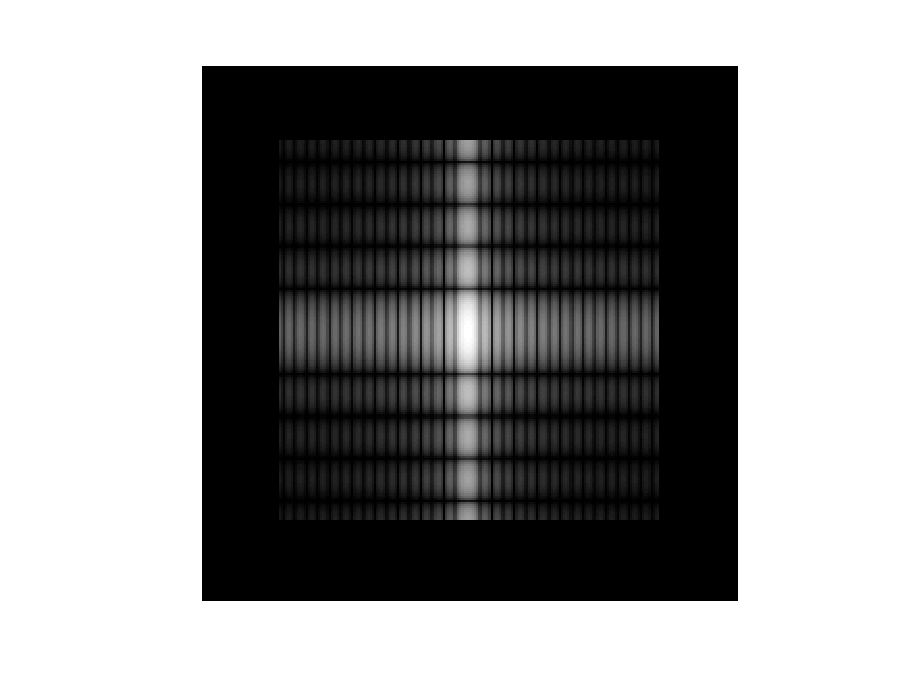
\includegraphics[width=\columnwidth]{Rotation_G_90_Fourier_Back.eps}
		\caption{\scriptsize Image rotated back by $90^{\circ}$.}
		\label{fig:rotated90Back}
		\end{subfigure}	
		
		\caption{Rotation.}
		\label{fig:rotation}
	\end{figure}
	\par Based on Figure \ref{fig:rotation}, we can conclude that a rotation angle of $\theta$ in spatial domain would give a rotation angle of $\theta$ in Fourier domain. However, the rotation of original image result in the loss of smoothness on the edges of the white rectangle especially in the case of $30^{\circ}$ and $60^{\circ}$. This gives the Fourier spectrum a wave-like grain.
	% \par The rotation property of discrete Fourier transform can be illustrated:
	% \begin{align}
	% 	F_{2}(x, y) &= F_{1}(x\cos(-\theta)+y\sin(-\theta), -x\sin(-\theta)+y\cos(-\theta)) \\
	% 	&= F_{1}(x\cos(\theta)-y\sin(\theta), x\sin(\theta)+y\cos(\theta))
	% \end{align}
\end{itemize}

\subsection*{1.8 Information in Fourier phase and magnitude}
\begin{itemize}
	\item \textbf{Question 13} What information is contained in the phase and in the magnitude of the Fourier transform?
	\begin{figure}[!ht]
		\footnotesize
		\centering 
		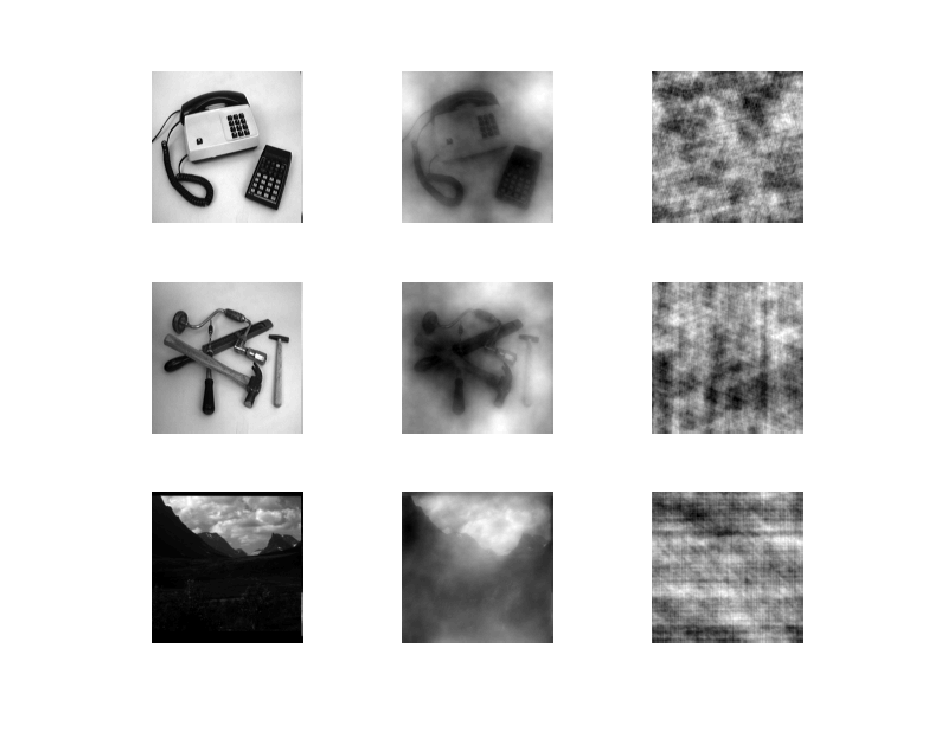
\includegraphics[width=\columnwidth]{Q13.eps}
		\caption{The first column are the original images. The second column contains the power spectrum for the images in the form of $\left|\hat{f}(\omega)\right|^{2} = \frac{1}{a |\omega|^{2}}$. The last column contains the random phase images.}
		\label{fig:Q13}
	\end{figure}
	\par From Figure \ref{fig:Q13}, we can see that the phase information is important for recognizing the feature of the image, since the second column of images have the same phase with the original images while different in magnitude. In contrast, the last column of images have the same magnitude with the original images while different in phase. However, its impossible to feature the images in the last column.
	\par Phase contains the phase difference between the sinusoid waves, thus could be used to determine the profile of the objects in the image. With phase being replaced by random values, the image could not be recognized any longer.
\end{itemize}

\section{Gaussian convolution implemented via FFT}
\subsection*{2.3 Filtering procedure}
\begin{itemize}
	\item \textbf{Question 14} Show the impulse response and variance for the above mentioned $t$-values. What are the variances of your discretized Gaussian kernel for $t$ = 0.1, 0.3, 1.0, 10.0 and 100.0?
	\par Figure \ref{fig:Q14} shows the impulse responses of the Gaussian kernel with different $t$. 
	\begin{figure}[!ht]
		\footnotesize
		\centering 
		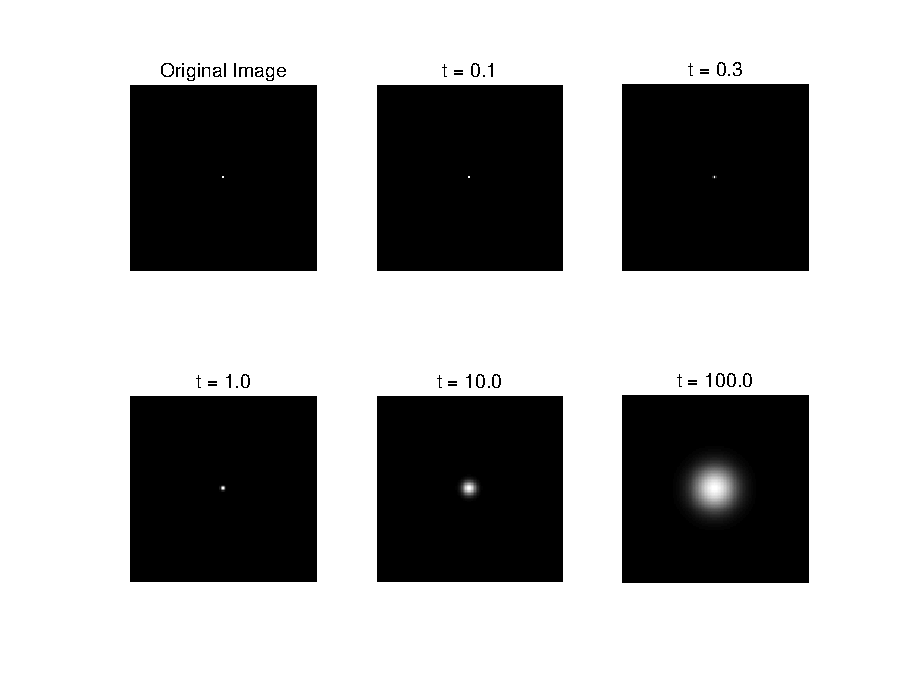
\includegraphics[width=0.8\columnwidth]{Q14.eps}
		\caption{Impulse response.}
		\label{fig:Q14}
	\end{figure}
	\par The variances for each $t$ are:
	\begin{align*}
	var_{t = 0.1} &= \begin{bmatrix} 0.0133 & 0.0000 \\ 0.0000 & 0.0133 \end{bmatrix} \\
	var_{t = 0.3} &= \begin{bmatrix} 0.2811 & 0.0000 \\ 0.0000 & 0.2811 \end{bmatrix} \\
	var_{t = 1.0} &= \begin{bmatrix} 1.0000 & 0.0000 \\ 0.0000 & 1.0000 \end{bmatrix} \\
	var_{t = 10.0} &= \begin{bmatrix} 10.0000 & 0.0000 \\ 0.0000 & 10.0000 \end{bmatrix} \\
	var_{t = 100.0} &= \begin{bmatrix} 100.0000 & 0.0000 \\ 0.0000 & 10.0000 \end{bmatrix}
	\end{align*}
	
	\item \textbf{Question 15} Are the results different from or similar to the estimated variance? How does the result correspond to the ideal continuous case? Lead: think of the relation between spatial and Fourier domains for different values of $t$.
	\par Referring to both Figure \ref{fig:Q14} and the variances, when $t=0.1$ and $t=0.3$ the results are different from the ideal continuous case. While, when $t \geq 1$, the result follows the ideal continuous case. The reason is when $t$ is too small, the impulse response would only be a pixel, thus the variance of would be different to the ideal case.
	
	\item \textbf{Question 16} Convolve a couple of images with Gaussian functions of different variances (like $t$ = 1.0, 4.0, 16.0, 64.0 and 256.0) and present your results. What effects can you observe?
	\par Figure \ref{fig:Q16Phone} and \ref{fig:Q16Few} show the result after applying Gaussian filter with various $t$ to \texttt{phonecalc128} and \texttt{few128}.	From the figures, we could conclude that the larger the $t$ is, the more blurry the image becomes. 
	\begin{figure}[!ht]
		\footnotesize
		\centering 
		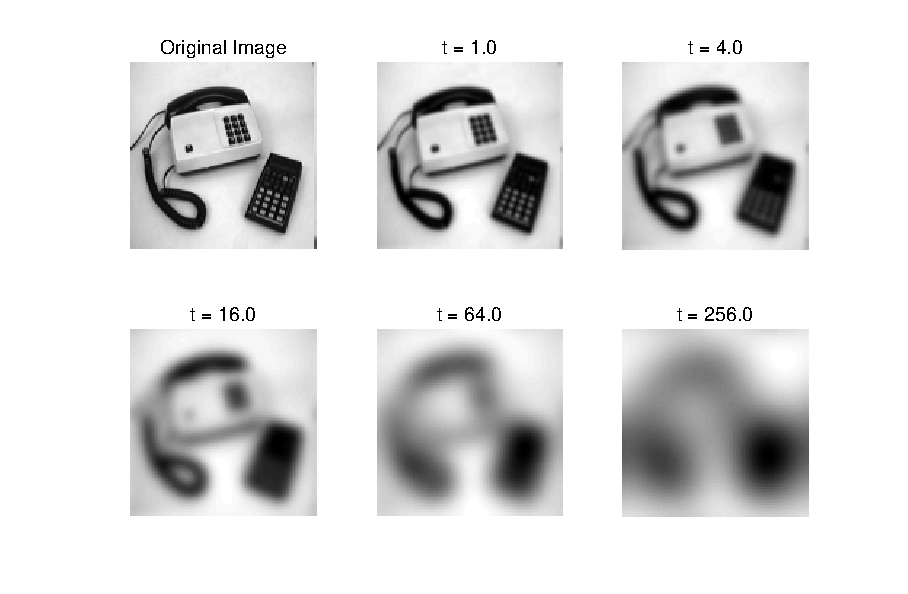
\includegraphics[width=0.8\columnwidth]{Q16_Phone.eps}
		\caption{\texttt{phonecalc128} with Gaussian filter.}
		\label{fig:Q16Phone}
	\end{figure}
	\begin{figure}[!ht]
		\footnotesize
		\centering 
		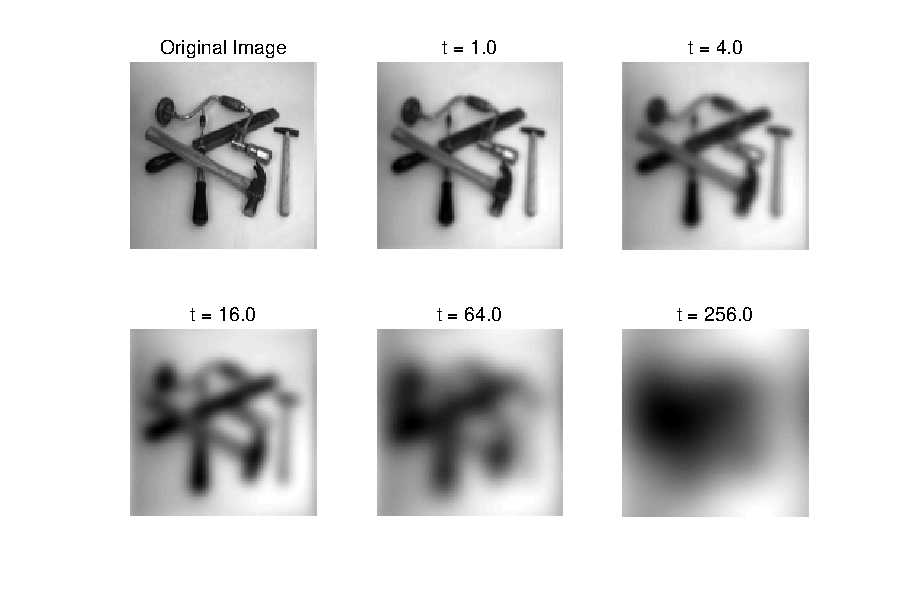
\includegraphics[width=0.8\columnwidth]{Q16_Few.eps}
		\caption{\texttt{few128} with Gaussian filter.}
		\label{fig:Q16Few}
	\end{figure}
%	\begin{figure}[!ht]
%		\footnotesize
%		\centering 
%		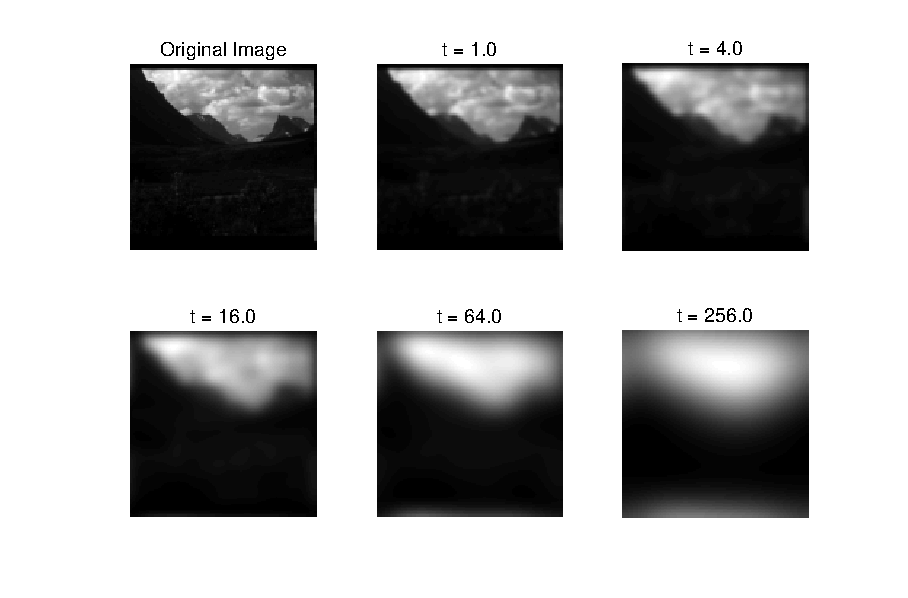
\includegraphics[width=0.8\columnwidth]{Q16_Nallo.eps}
%		\caption{\texttt{nallo128} with Gaussian filter.}
%		\label{fig:Q16Nallo}
%	\end{figure}
\end{itemize}

\section{Smoothing}
\subsection*{3.1 Smoothing of noisy data}
\par The original image of \texttt{office256} and its noisy images are shown in Figure \ref{fig:officeAndNoisyOffice}.
\begin{figure}[!ht]
	\centering 
	\begin{subfigure}[t]{.32\linewidth} % .32 for three polts .49 for two plots
		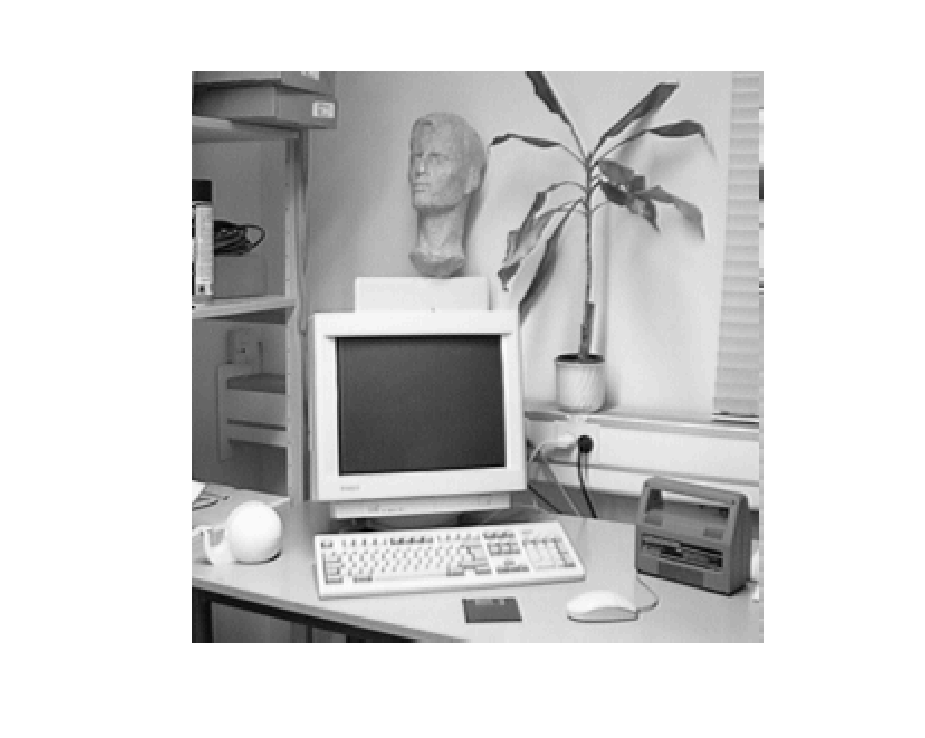
\includegraphics[width=0.95\columnwidth]{Office.eps}
		\caption{\scriptsize Original image.}
		\label{fig:office}
	\end{subfigure}
	\begin{subfigure}[t]{.32\linewidth} % .32 for three polts .49 for two plots
		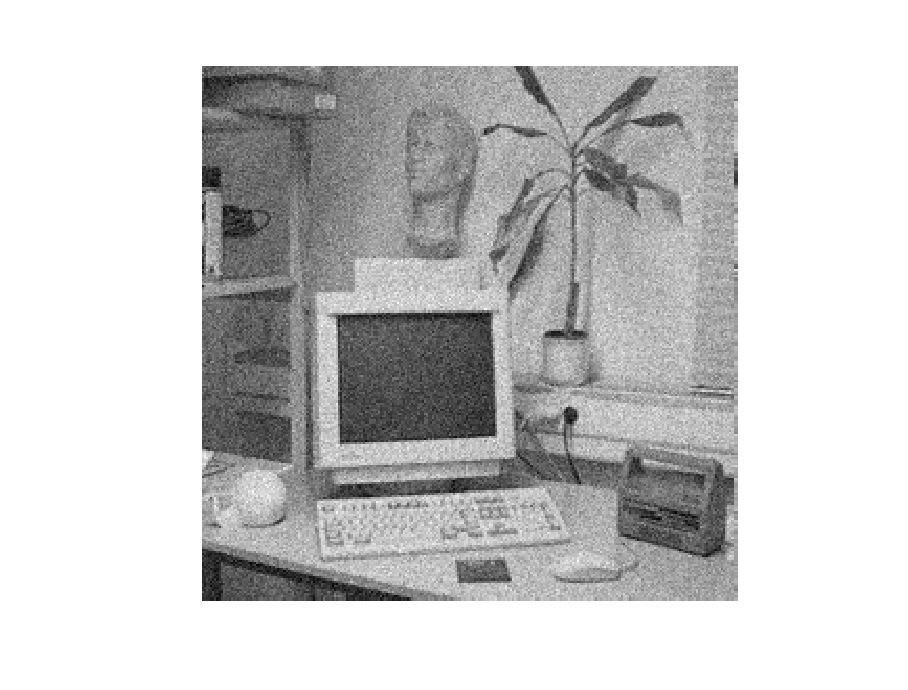
\includegraphics[width=\columnwidth]{Office_Gauss_Noise.eps}
		\caption{\scriptsize Image with Gaussian noise.}
		\label{fig:officeGauss}
	\end{subfigure}
	\begin{subfigure}[t]{.32\linewidth} % .32 for three polts .49 for two plots
		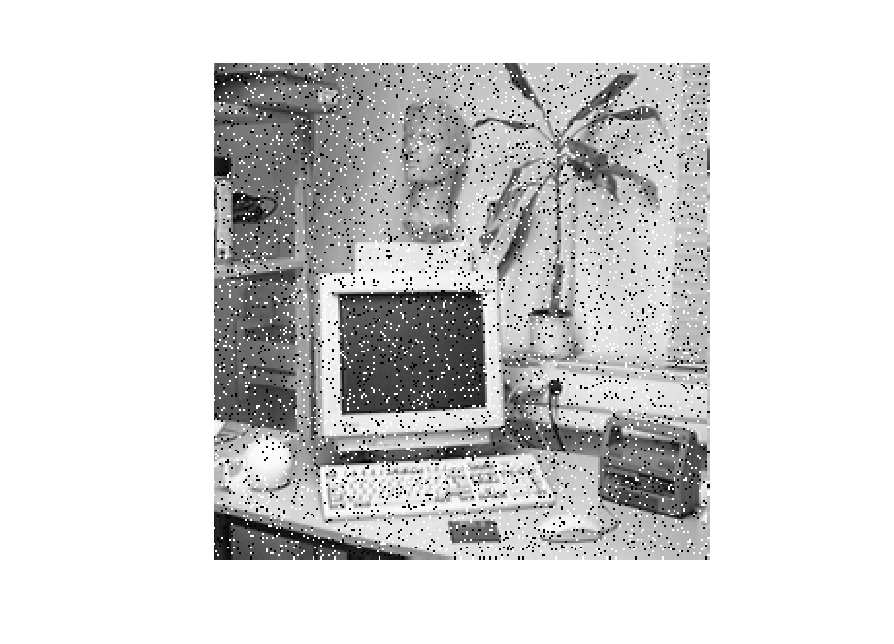
\includegraphics[width=1.05\columnwidth]{Office_Sap_Noise.eps}
		\caption{\scriptsize Image with Salt-and-pepper noise.}
		\label{fig:officeSap}
	\end{subfigure}

	\caption{Original image and image with noise.}
	\label{fig:officeAndNoisyOffice}
\end{figure}

\begin{itemize}
	\item \textbf{Question 17} What are the positive and negative effects for each type of filter? Describe what you observe and name the effects that you recognize. How do the results depend on the filter parameters? Illustrate with MATLAB figure(s).
	\par The result of Gaussian filter, median filter and ideal low-pass filter are shown in Figure \ref{fig:gauss}, \ref{fig:med}, and \ref{fig:lowpass} correspondingly.
	\begin{figure}[!ht]
		\centering 
		\begin{subfigure}[t]{.32\linewidth} % .32 for three polts .49 for two plots
			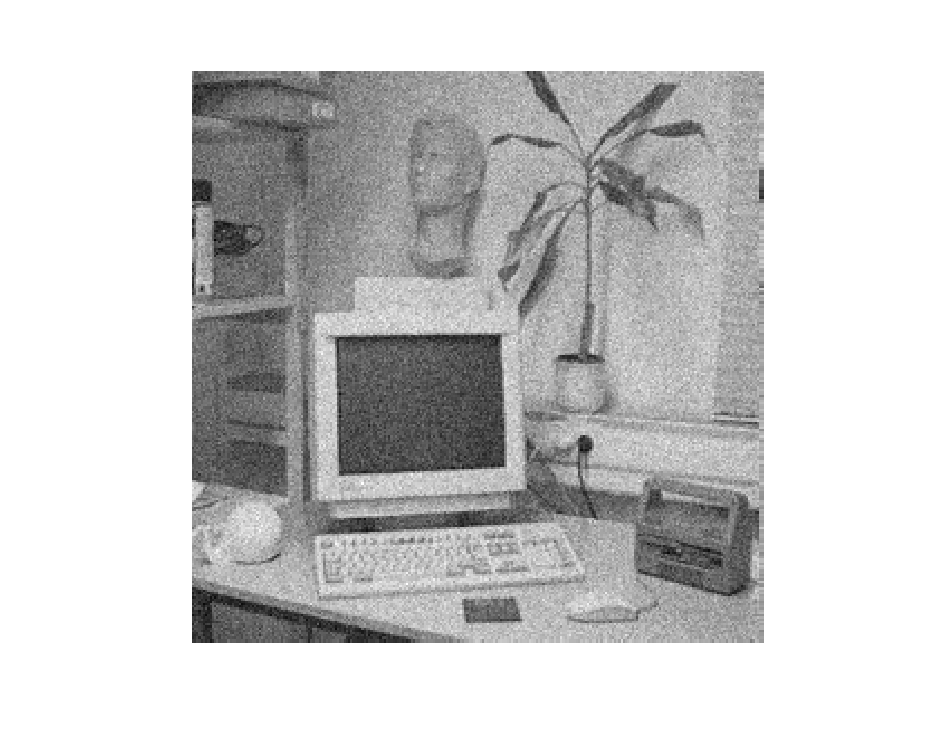
\includegraphics[width=\columnwidth]{Q17_Gauss_to_Gauss_0_1.eps}
			\caption{\scriptsize Gaussian filtering to Gaussian noise with variance 0.1.}
			\label{fig:gaussToGauss0.1}
		\end{subfigure}
		\begin{subfigure}[t]{.32\linewidth} % .32 for three polts .49 for two plots
			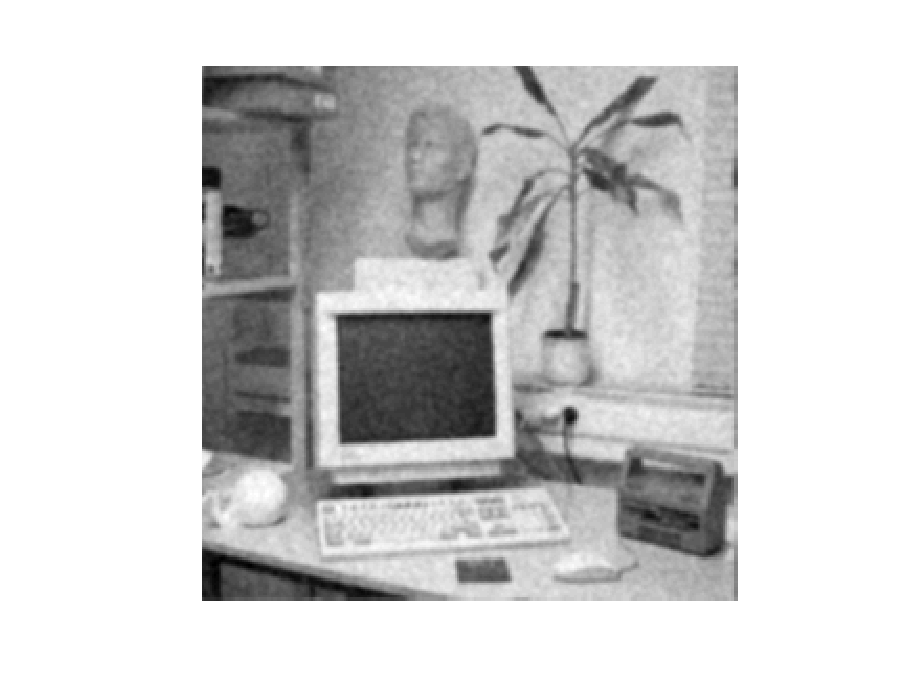
\includegraphics[width=\columnwidth]{Q17_Gauss_to_Gauss_1.eps}
			\caption{\scriptsize Gaussian filtering to Gaussian noise with variance 1.}
			\label{fig:gaussToGauss1}
		\end{subfigure}
		\begin{subfigure}[t]{.32\linewidth} % .32 for three polts .49 for two plots
			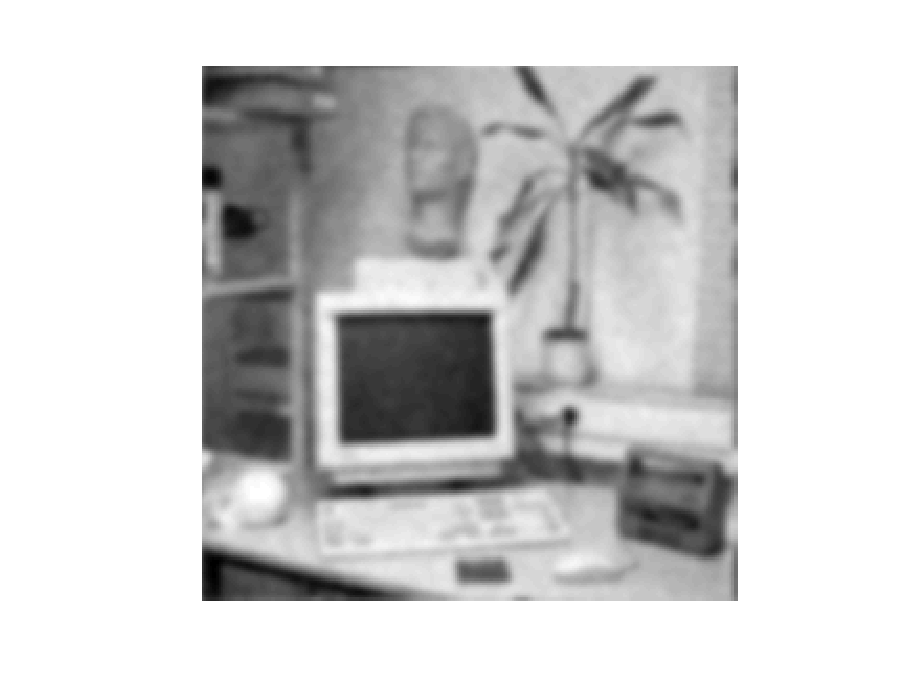
\includegraphics[width=\columnwidth]{Q17_Gauss_to_Gauss_4.eps}
			\caption{\scriptsize Gaussian filtering to Gaussian noise with variance 4.}
			\label{fig:gaussToGauss4}
		\end{subfigure}

		\begin{subfigure}[t]{.32\linewidth} % .32 for three polts .49 for two plots
			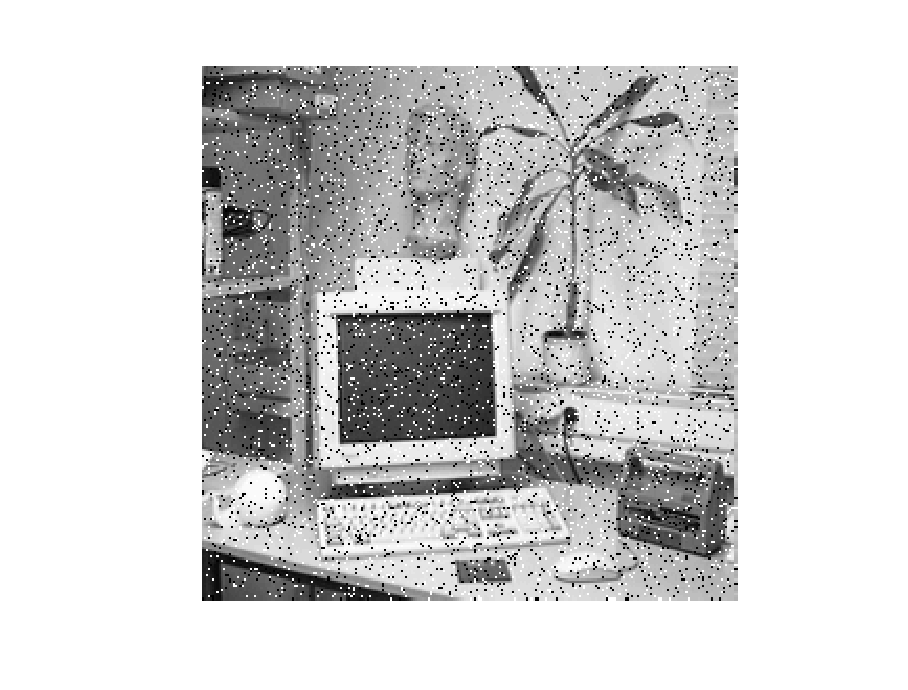
\includegraphics[width=\columnwidth]{Q17_Gauss_to_Sap_0_1.eps}
			\caption{\scriptsize Gaussian filtering to Salt-and-pepper noise with variance 0.1.}
			\label{fig:gaussToSap0.1}
		\end{subfigure}
		\begin{subfigure}[t]{.32\linewidth} % .32 for three polts .49 for two plots
			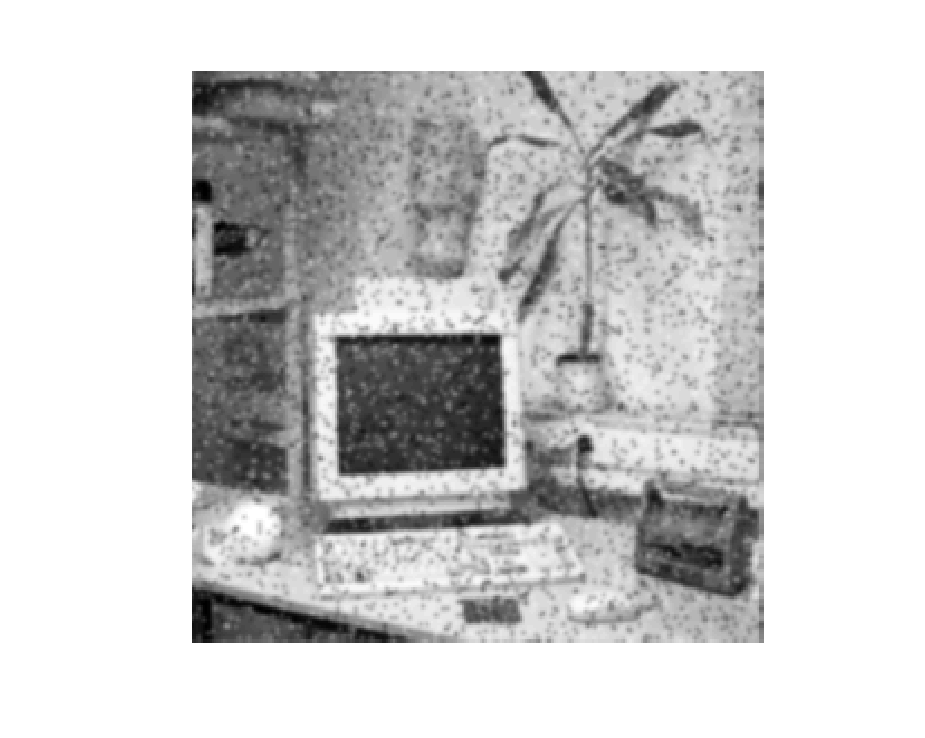
\includegraphics[width=\columnwidth]{Q17_Gauss_to_Sap_1.eps}
			\caption{\scriptsize Gaussian filtering to Salt-and-pepper noise with variance 1.}
			\label{fig:gaussToSap1}
		\end{subfigure}
		\begin{subfigure}[t]{.32\linewidth} % .32 for three polts .49 for two plots
			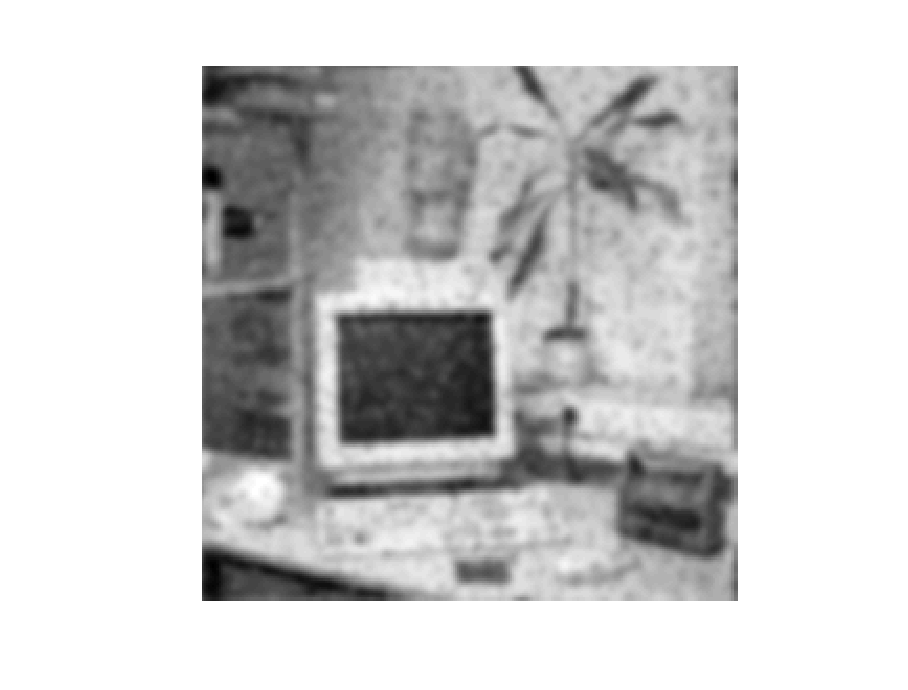
\includegraphics[width=\columnwidth]{Q17_Gauss_to_Sap_4.eps}
			\caption{\scriptsize Gaussian filtering to Salt-and-pepper noise with variance 4.}
			\label{fig:gaussToSap4}
		\end{subfigure}

		\caption{Gaussian filtering.}
		\label{fig:gauss}
	\end{figure}
	
	\begin{itemize}
		\item Gaussian smoothing blurs the image to reduce noise obviously and is very effective in removing Gaussian noise. However, with the variance increases, the image loses detail. The performance in smoothing the image with Salt-and-pepper noise is not so good as Median filter, the ``salt'' and ``pepper'' pixels are blurred but still obvious.
		\item Median filtering is very effective in removing Salt-and-pepper noise as we can see from Figure \ref{fig:medToSap2*2}, the $2\times 2$ window size of median filter removes all the Salt-and-pepper pixels of the image. Also, the edges of the images are still relatively sharp in the median filtering cases. However, median filtering loses details very quickly when the window size becomes bigger.
		\item Ideal low-pass filtering performs worst behavior in both types of noise. If the cut-off frequency is low, then all the moderate and high frequency would be removed, thus becoming more likely to have sinusiod like output image based on the theory from Section 1. While, if the cut-off frequency is high, then small change would be applied to the noise.
	\end{itemize}

	\begin{figure}[!ht]
		\centering 
		\begin{subfigure}[t]{.32\linewidth} % .32 for three polts .49 for two plots
			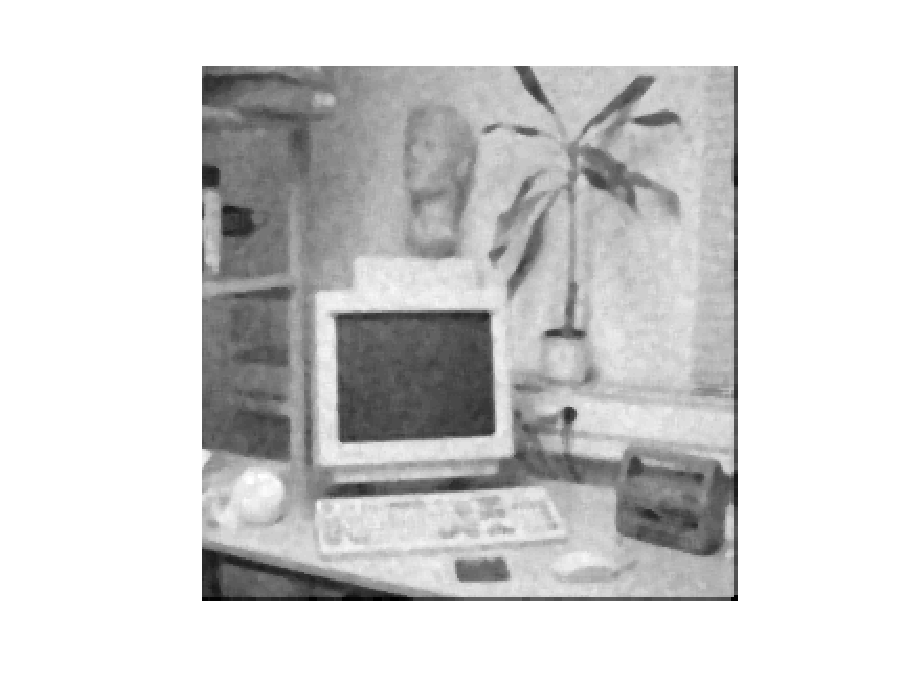
\includegraphics[width=\columnwidth]{Q17_Med_to_Gauss_2_2.eps}
			\caption{\scriptsize Median filtering to Gaussian noise with window size 2$\times$2.}
			\label{fig:medToGauss2*2}
		\end{subfigure}
		\begin{subfigure}[t]{.32\linewidth} % .32 for three polts .49 for two plots
			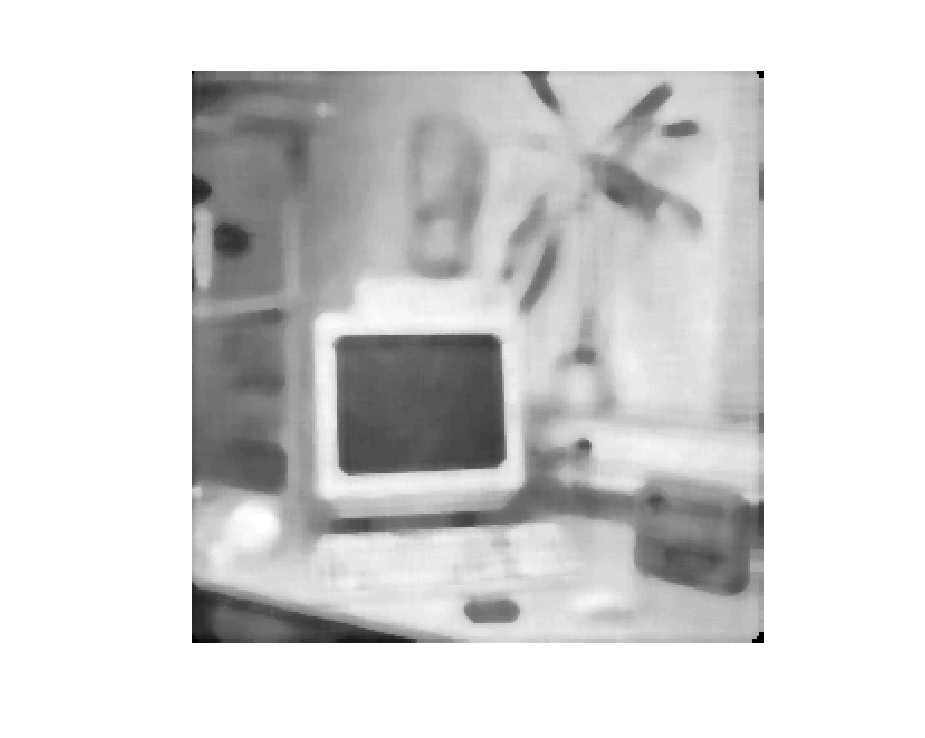
\includegraphics[width=\columnwidth]{Q17_Med_to_Gauss_3_3.eps}
			\caption{\scriptsize Median filtering to Gaussian noise with window size 3$\times$3.}
			\label{fig:medToGauss3*3}
		\end{subfigure}
		\begin{subfigure}[t]{.32\linewidth} % .32 for three polts .49 for two plots
			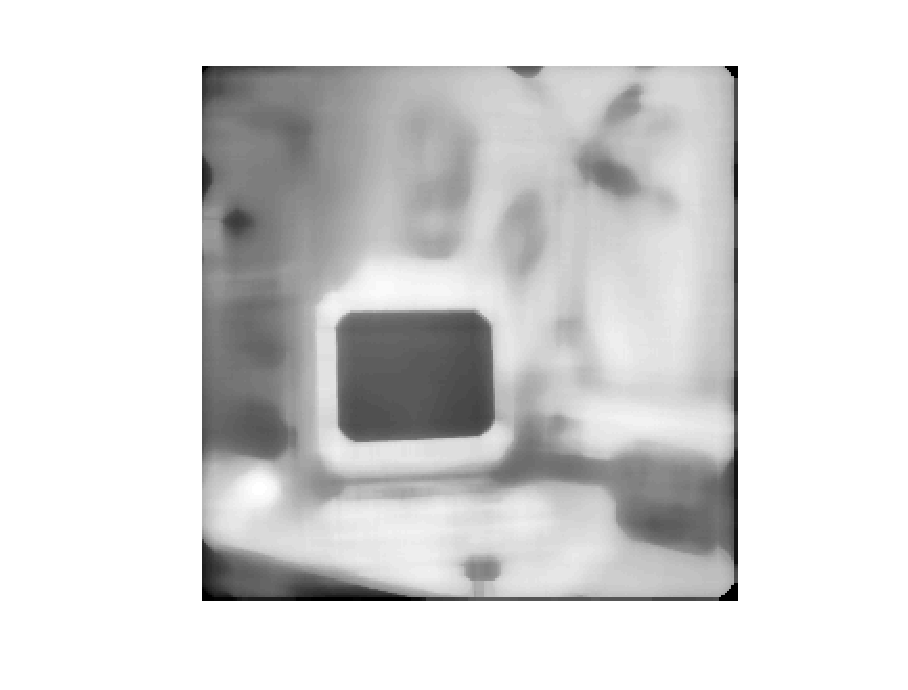
\includegraphics[width=\columnwidth]{Q17_Med_to_Gauss_4_4.eps}
			\caption{\scriptsize Median filtering to Gaussian noise with window size 4$\times$4.}
			\label{fig:medToGauss4*4}
		\end{subfigure}

		\begin{subfigure}[t]{.32\linewidth} % .32 for three polts .49 for two plots
			\includegraphics[width=\columnwidth]{Q17_Med_to_Sap_2_2.eps}
			\caption{\scriptsize Median filtering to Salt-and-pepper noise with window size 2$\times$2.}
			\label{fig:medToSap2*2}
		\end{subfigure}
		\begin{subfigure}[t]{.32\linewidth} % .32 for three polts .49 for two plots
			\includegraphics[width=\columnwidth]{Q17_Med_to_Sap_3_3.eps}
			\caption{\scriptsize Median filtering to Salt-and-pepper noise with window size 3$\times$3.}
			\label{fig:medToSap3*3}
		\end{subfigure}
		\begin{subfigure}[t]{.32\linewidth} % .32 for three polts .49 for two plots
			\includegraphics[width=\columnwidth]{Q17_Med_to_Sap_4_4.eps}
			\caption{\scriptsize Median filtering to Salt-and-pepper noise with window size 4$\times$4.}
			\label{fig:medToSap4*4}
		\end{subfigure}

		\caption{Median filtering.}
		\label{fig:med}
	\end{figure}	

	\begin{figure}[!ht]
		\centering 
		\begin{subfigure}[t]{.32\linewidth} % .32 for three polts .49 for two plots		
			\includegraphics[width=\columnwidth]{Q17_Lowpass_to_Gauss_0_1.eps}
			\caption{\scriptsize Ideal low-pass filtering to Gaussian noise with cut-off frequency 0.1.}
			\label{fig:lowpassToGauss0.1}
		\end{subfigure}
		\begin{subfigure}[t]{.32\linewidth} % .32 for three polts .49 for two plots
			\includegraphics[width=\columnwidth]{Q17_Lowpass_to_Gauss_0_25.eps}
			\caption{\scriptsize Ideal low-pass filtering to Gaussian noise with cut-off frequency 0.25.}
			\label{fig:lowpassToGauss0.25}
		\end{subfigure}
		\begin{subfigure}[t]{.32\linewidth} % .32 for three polts .49 for two plots
			\includegraphics[width=\columnwidth]{Q17_Lowpass_to_Gauss_0_5.eps}
			\caption{\scriptsize Ideal low-pass filtering to Gaussian noise with cut-off frequency 0.5.}
			\label{fig:lowpassToGauss0.5}
		\end{subfigure}

		\begin{subfigure}[t]{.32\linewidth} % .32 for three polts .49 for two plots
			\includegraphics[width=\columnwidth]{Q17_Lowpass_to_Sap_0_1.eps}
			\caption{\scriptsize Ideal low-pass filtering to Salt-and-pepper noise with cut-off frequency 0.1.}
			\label{fig:lowpassToSap0.1}
		\end{subfigure}
		\begin{subfigure}[t]{.32\linewidth} % .32 for three polts .49 for two plots
			\includegraphics[width=\columnwidth]{Q17_Lowpass_to_Sap_0_25.eps}
			\caption{\scriptsize Ideal low-pass filtering to Salt-and-pepper noise with cut-off frequency 0.25.}
			\label{fig:lowpassToSap0.25}
		\end{subfigure}
		\begin{subfigure}[t]{.32\linewidth} % .32 for three polts .49 for two plots
			\includegraphics[width=\columnwidth]{Q17_Lowpass_to_Sap_0_5.eps}
			\caption{\scriptsize Ideal low-pass filtering to Salt-and-pepper noise with cut-off frequency 0.5.}
			\label{fig:lowpassToSap0.5}
		\end{subfigure}

		\caption{Ideal low-pass filtering.}
		\label{fig:lowpass}
	\end{figure}
	
	\item \textbf{Question 18} What conclusions can you draw from comparing the results of the respective methods?
	\par Gaussian smoothing is effective in removing Gaussian noise. Median filtering is effective in removing Salt-and-pepper noise. Both of Gaussian filter and ideal low-pass filter decrease the highest frequency of the image thus blurring the image in result. Higher variance of Gaussian filter in spatial domain, the lower the variance in the Fourier domain, which resulting in more high frequencies being discarded. Ideal low-pass filter remove the frequency that is higher than the cut-off frequency in the Fourier domain thus resulting in the ``ringing'' effect.
\end{itemize}

\subsection*{3.2 Smoothing and sub-sampling}
\begin{itemize}
	\item \textbf{Question 19} What effects do you observe when sub-sampling the original image and the smoothed variants? Illustrate both filters with the best results found for iteration $i$ = 4.
	\par Figure \ref{fig:smoothingSampling} illustrate the sub-sampled images and the smoothed variants with Gaussian smoothing of variance 0.5 and ideal low-pass filtering of frequency 0.25. The Gaussian filter blurs the image while the ideal low-pass filter brings sinusoid texture to the image. Sub-sampling would make the pixels bigger and use one pixel to replace four pixels before sub-sampling. Since the loss of values, the image becomes rough. Higher resolution image contains more details after smoothing and filtering. Moreover, smoothing before sub-sampling introduces smoother edges to the image.
	
	\item \textbf{Question 20} What conclusions can you draw regarding the effects of smoothing when combined with sub-sampling? Hint: think in terms of frequencies and side effects.
	\par Smoothing and filtering with Gaussian or ideal low-pass filter decreases highest frequency of the image, thus preventing aliasing before sampling. Also, in this way, the side effects are decreased so that aliasing is less likely to take place.
	
	\begin{figure}[!ht]
		\footnotesize
		\centering 
		\includegraphics[width=\columnwidth]{Smoothing_Subsampling_Gauss_0_5_Lowpass_0_25.eps}
		\caption{The first two rows contain the images with just sub-sampling and their Fourier spectrum. The second two rows contain the images with Gaussian smoothing and sub-sampling and their Fourier spectrum with variance 0.5. The last two rows contain the images with ideal low-pass filtering and sub-sampling and their Fourier spectrum with cut-off frequency 0.25. The first column of images are all original and their spectrum.}
		\label{fig:smoothingSampling}
	\end{figure}
\end{itemize}

% Template
%%%%%%%%%%%%%%%%%%%%%%%%%%%%%%%%%%%%%%%%
% \lstinputlisting{fftwave.m}
%%%%%%%%%%%%%%%%%%%%%%%%%%%%%%%%%%%%%%%%
\end{document}